%%%%%%%%%%%%%%%%%%%%%%%%%%%%%%%%%%%%%%%%%%%%%%%%%%%%%%%%%%%%%%%%%%%%%%%%%%%%%%%%
%2345678901234567890123456789012345678901234567890123456789012345678901234567890
%        1         2         3         4         5         6         7         8

%\documentclass[final,letterpaper, 10 pt, conference]{ieeeconf}  % Comment this line out if you need a4paper

\documentclass[10pt, conference, compsocconf]{IEEEtran}
%\documentclass[a4paper, 10pt, conference]{ieeeconf}      % Use this line for a4 paper

\IEEEoverridecommandlockouts                              % This command is only needed if
                                                          % you want to use the \thanks command

\newcommand{\eu}{\textrm{e}}
\newcommand{\figref}[1]{Fig.~\ref{fig:#1}}
\overrideIEEEmargins
\usepackage[obeyFinal]{todonotes}
\RequirePackage{graphicx}
\usepackage{subfigure}
\usepackage{bm}
%\usepackage{subequation}
\graphicspath{ {figures/} }
\usepackage{url}
%\usepackage[tight,footnotesize]{subfigure}
\usepackage{fainekos-macros}
\newcommand{\hatodo}[1]{\todo{HA: #1}}
\newcommand{\hatodoin}[1]{\todo[inline]{HA: #1}}
\newcommand{\sAccu}{\epsilon}
\newcommand{\sDelay}{\delta}
\newcommand{\de}{(\sDelay,\sAccu)}
\newcommand{\dek}[1]{(\sDelay_{#1},\sAccu_{#1})}
\newcommand{\hWc}{\widehat{\Wc}}
\newcommand{\sDelayV}{\underline{\sDelay}}
\newcommand{\sAccuV}{\underline{\sAccu}}
\newcommand{\ESet}{\mathcal{E}}
%\newcommand{\bm}{\hat{B}}
\newcommand{\MPCProb}[1]{\mathbb{P_{#1}}}
\newcommand{\RAMPCProb}[2]{\mathbb{P}_{#1}(\hat{\stPt}_{#2},\sDelay_{#2},\sAccu_{#2},\inpPt_{#2 -1})}
\global\long\def\ZSet{\Zc}
\global\long\def\Cc{\mathcal{C}}
\global\long\def\Nom#1{\overline{#1}}
\newcommand{\bla}[1]{\overbar{#1}}
\newcommand{\bli}[1]{\overline{BLI #1}}
\newboolean{TECH_REPORT}
\setboolean{TECH_REPORT}{FALSE}
\newcommand{\Given}{|}

\usepackage{array}
\usepackage{url}

\newcommand\Mark[1]{\textsuperscript#1}


% See the \addtolength command later in the file to balance the column lengths
% on the last page of the document

% The following packages can be found on http:\\www.ctan.org
%\usepackage{graphics} % for pdf, bitmapped graphics files
%\usepackage{epsfig} % for postscript graphics files
%\usepackage{mathptmx} % assumes new font selection scheme installed
%\usepackage{times} % assumes new font selection scheme installed
\usepackage{amsmath} % assumes amsmath package installed
\usepackage{amssymb}  % assumes amsmath package installed
\begin{document}
\title{\LARGE \bf
Co-Design of Anytime Computation and Robust Control
}
%
\author{Yash Vardhan Pant, Kartik Mohta, Houssam Abbas, Truong X. Nghiem, Joseph Devietti, Rahul Mangharam% <-this % stops a space
\thanks{*This work was supported by STARnet a Semiconductor Research
Corporation program sponsored by MARCO and DARPA.}% <-this % stops a space
\thanks{The Departments of Electrical and Systems Engineering and Computer and Information Sciences, University of Pennsylvania, Philadelphia, U.S.A.
        {\tt\small
        \{yashpant,kmohta,habbas,nghiem,rahulm\}@seas.upenn.edu, devietti@cis.upenn.edu}}%
}


%\author{\IEEEauthorblockN{Yash Vardhan Pant, Houssam Abbas, Kartik Mohta, Rahul Mangharam}
%\IEEEauthorblockA{The Department of Electrical  \\ and Systems Engineering, \\
%University of Pennsylvania, \\
%Philadelphia, U.S.A\\
%yashpant@seas.upenn.edu, kmohta@seas.upenn.edu, \\habbas@seas.upenn.edu, rahulm@seas.upenn.edu}
%\and
%\IEEEauthorblockN{Joseph Devietti}
%\IEEEauthorblockA{The Department of Computer\\  and Information Sciences, \\
%University of Pennsylvania, \\
%Philadelphia, U.S.A\\
%devietti@cis.upenn.edu}
%}




%\begin{document}

\maketitle
\thispagestyle{empty}
\pagestyle{empty}

\ifthenelse{\boolean{TECH_REPORT}}
{
	\section*{Appendix}
\label{appendix}

In this appendix we give the detailed mathematical derivation of the results of Section \ctrlProbSecRef.
The controller is designed using a Robust Model Predictive
Control (RMPC) approach via constraint restriction \cite{richardsetal05rmp, chiscietal01swp}, 
and augments it by an adaptation to the error-delay curve of the estimator.
In order to ensure robust safety and feasibility, the key idea of
the RMPC approach is to tighten the constraint sets iteratively to account
for possible effect of the disturbances. 
As time progresses, this ``robustness
margin'' is used in the MPC optimization with the nominal dynamics,
i.e., the original dynamics where the disturbances are either removed
or replaced by nominal disturbances.
%An advantage of this approach is that, 
Because only the nominal dynamics are used, the complexity of the optimization is the same as for the nominal problem.

Since the controller only has access to the estimated state $\hat{x}$, we need
to rewrite the plant's dynamics with respect to $\hat{x}$. 
The error
between $ $$x_{k}$ and $\hat{x}_{k}$ is $e_{k}=x_{k}-\hat{x}_{k}$.
At time step $k+1$ we have
\begin{align*}
\hat{x}_{k+1} & =x_{k+1}-e_{k+1}\\
 & =Ax_{k}+B_{1}(\sDelay_k)u_{k-1}+B_{2}(\sDelay[k])u_{k}+w_{k}-e_{k+1}\text{,}
\end{align*}
 then, by writing $x_{k}=\hat{x}_{k}+e_{k}$, we obtain the dynamics
\begin{equation}
\hat{x}_{k+1}=A\hat{x}_{k}+B_{1}(\sDelay[k])u_{k-1}+B_{2}(\sDelay[k])u_{k}+\hat{w}_{k}\label{eq:estimator-dynamics}
\end{equation}
 where $\hat{w}_{k}=w_{k}+Ae_{k}-e_{k+1}$.
The set of possible values of $\hat{w}_{k}$
depends on the estimation accuracy at steps $k$ and $k+1$ and is
denoted by $\hWc(\sAccu[k],\sAccu[k+1])$, i.e.,
$\hWc(\sAccu,\sAccu')\defeq \left\{ w+Ae-e'\sut w\in\Wc,e\in\ESet(\sAccu),e'\in\ESet(\sAccu')\right\}$.
Note that %we assume
$\hWc(\sAccu[k],\sAccu[k+1])$ is independent
of the time step $k$. %
It can be computed as $\hWc(\sAccu,\sAccu')=\Wc\oplus A\ESet(\sAccu)\oplus\left(-\ESet(\sAccu')\right)$
where the symbol $\oplus$ denotes the Minkowski sum of two sets.

The dynamics in \eqref{eq:estimator-dynamics} has a non-standard form
where it depends on both the current and the previous control inputs.
However we can expand the state variable to store the previous control
input as
\[
\hat{z}_{k}=\begin{bmatrix}\hat{x}_{k}\\
u_{k-1}
\end{bmatrix}\in\Re^{n+m}
\]
and rewrite the dynamics as, for all $k\geq0$,
\begin{equation}
\hat{z}_{k+1}=\hat{A}(\sDelay_k)\hat{z}_{k}+\hat{B}(\sDelay_k)u_{k}+\hat{F}\hat{w}_{k}\text{.}\label{eq:estimator-std-dynamics}
\end{equation}
Here, the system matrices are
\begin{equation}
\begin{gathered}
\hat{A}(\sDelay_k)=\begin{bmatrix}A & B_{1}(\sDelay_k)\\
\bm{0}_{m\times n} & \bm{0}_{m\times m}
\end{bmatrix},\\
\hat{B}(\sDelay_k)=\begin{bmatrix}B_{2}(\sDelay_k)\\
\IdentityMatrix_{m}
\end{bmatrix},\quad\hat{F}=\begin{bmatrix}\IdentityMatrix_{n}\\
\bm{0}_{m\times n}
\end{bmatrix}\text{.}
\end{gathered}
\label{eq:lifted-matrices}
\end{equation}

Let the actual expanded state be $z_{k}=\left[x_{k}^{T},u_{k-1}^{T}\right]^{T}$.
Because the expanded state consists of both the plant's state and
the previous control input, the state constraint $x_{k}\in\stSet$
and the control constraint $u_{k}\in\inpSet$ are equivalent to the
joint constraint $z_{k}\in\stSet\times\inpSet$. We can now describe
the RAMPC algorithm for the dynamics in \eqref{eq:estimator-std-dynamics}.

\subsection{Tractable RAMPC Algorithm}

Let $N\geq1$ be the horizon length of the RMPC optimization. 
Because the system
matrices in the state equation~(\ref{eq:estimator-std-dynamics})
depend nonlinearly on the variables $\sDelay_k$, the RMPC optimization
is generally a mixed-integer nonlinear program, which is very hard
to solve. To simplify the RMPC optimization to make it tractable, we fix the estimation mode for the entire RMPC horizon.

Let $\RAMPCProb{\de}{k}$
denote the RMPC optimization problem at step $k\geq0$ where the current
state estimate is $\hat{x}_{k}$, the current estimation mode is $(\sDelay_k,\sAccu_k)\in\Delta$,
the previous control input is $u_{k-1}$, and the estimation mode
for the entire horizon (after step $k$) is fixed at $(\sDelay,\sAccu)\in\Delta$.
Since the system matrices become constant now, if the stage cost $\ell(\cdot)$
is linear or positive semidefinite quadratic, each optimization problem
$\RAMPCProb{\de}{\cdot}$ is tractable and can be solved
efficiently as we will show later. 
The RAMPC algorithm with Anytime Estimation is stated in Alg. \algoref.

\subsection{RMPC Formulation}

We formulate the RMPC optimization $\RAMPCProb{\de}{k}$
with respect to the nominal dynamics, which is the original dynamics
in \eqref{estimator-std-dynamics} but the disturbances are either
removed or replaced by nominal disturbances. 
To ensure robust feasibility
and safety, the state constraint set is tightened after each step
using a candidate stabilizing state feedback control, and a terminal
constraint is derived. 
In this RMPC formulation, we extend the approach
in \cite{richardsetal05rmp, chiscietal01swp}. 
At time step $k$, given
$(\hat{x}_{k},\sDelay_k,\sAccu_k,u_{k-1})$ and for a fixed $(\sDelay,\sAccu)$,
we solve the following optimization 

\begin{subequations}
	\label{eq:RMPC1}
 \begin{equation} J_{\sDelay,\sAccu}^{*} \left(\hat{x}_{k},\sDelay_k,\sAccu_k,u_{k-1}\right) = \min_{\boldsymbol{u},\boldsymbol{x}}\sum_{j=0}^{N}\ell(\Nom x_{k+j\Given k},u_{k+j\Given k})
 \end{equation}
 \begin{equation}
  \text{subject to, }\forall j\in\left\{ 0,\dots,N\right\} \nonumber 
 \end{equation}
 \begin{equation}
  \Nom z_{k+j+1\Given k}=\hat{A}(\sDelay_{k+j\Given k})\Nom z_{k+j\Given k}+\hat{B}(\sDelay_{k+j\Given k})u_{k+j\Given k}\label{eq:RMPC1-dyn}
 \end{equation}
 \begin{equation}
  ( \sDelay_{k+j+1\Given k},\sAccu_{k+j+1\Given k} ) \!=\! (\sDelay,\sAccu ) \nonumber
 \end{equation}
 \begin{equation}
  (\sDelay_{k\Given k},\sAccu_{k\Given k}) \!=\! (\sDelay_k,\sAccu_k)  \label{eq:RMPC1-delay}
 \end{equation}
 \begin{equation}
  \Nom x_{k+j\Given k}=\begin{bmatrix}\IdentityMatrix_{n} \quad \bm{0}_{n\times m}\end{bmatrix}\Nom z_{k+j\Given k}\label{eq:RMPC1-z2x}
 \end{equation}
 \begin{equation}
  \Nom z_{k\Given k}=\left[\hat{x}_{k}^{T},u_{k-1}^{T}\right]^{T} \label{eq:RMPC1-z0}
 \end{equation}
 \begin{equation}
  \Nom z_{k+j\Given k}\in\ZSet_{j}\left(\sAccu_k,\sAccu\right)\label{eq:RMPC1-zset}
 \end{equation}
 \begin{equation}
  \Nom z_{k+N+1\Given k}\in\ZSet_{f}\left(\sAccu_k,\sAccu\right) \label{eq:RMPC1-zfinalset}
  \end{equation}
\end{subequations} 

in which $\Nom z$ and $\Nom x$
are the variables of the nominal dynamics. The constraints of the
optimization are explained below.
\begin{itemize}
\item \eqref{eq:RMPC1-dyn} is the nominal dynamics.
\item \eqref{eq:RMPC1-delay} states that the estimation mode is fixed at $\left(\sDelay,\sAccu\right)$
except for the first time step when it is $\left(\sDelay_k,\sAccu_k\right)$.
\item \eqref{eq:RMPC1-z2x} extracts the nominal state $\Nom x$ of the plant
from the nominal expanded state $\Nom z$.
\item \eqref{eq:RMPC1-z0} initializes the nominal expanded state at time step
$k$ by stacking the current state estimate and the previous control
input.
\item \eqref{eq:RMPC1-zset} tightens the admissible set of the nominal expanded
states by a sequence of shrinking sets.
\item \eqref{eq:RMPC1-zfinalset} constrains the terminal expanded state to
the terminal constraint set $\ZSet_{f}$.
\end{itemize}

\noindent\textit{The state constraint $\ZSet_{j}$:}
%
The tightened state constraint sets $\ZSet_{j}\left(\sAccu_k,\sAccu\right)$
are parameterized with two parameters $\sAccu_k$ and $\sAccu$.
They are defined as follows, for all $j\in\left\{ 0,\dots,N\right\} $
\begin{eqnarray}
\ZSet_{0}(\sAccu_k,\sAccu)=\ZSet\ominus\hat{F} \ESet(\sAccu_k)\label{eq:RMPC1-Z0}
\\
\ZSet_{j+1}(\sAccu_k,\sAccu)=\ZSet_{j}(\sAccu,\sAccu)\ominus L_{j}\hat{F}\hWc(\sAccu_k,\sAccu)\label{eq:RMPC1-Zj}
\label{eq:RMPC1-Z}
\end{eqnarray} 
in which the symbol $\ominus$
denotes the Pontryagin difference between two sets. The set $\ZSet$
combines the constraints for both the plant's state and the control
input: $\ZSet=\stSet\times\inpSet$. The matrix $L_{j}$ is the state
transition matrix for the nominal dynamics in \eqref{eq:RMPC1-dyn} under
a candidate state feedback gain $K_{j}(\sDelay)$, for $j\in\left\{ 0,\dots,N\right\}$
\begin{eqnarray}
\label{eq:RMPC1-L}
L_{0}=\IdentityMatrix\label{eq:RMPC1-L0}\\
L_{j+1}=(\hat{A}(\sDelay)+\hat{B}(\sDelay)K_{j}(\sDelay))L_{j}\label{eq:RMPC1-Lj}
\end{eqnarray}
Note that the possibly time-varying sequence $K_{j}(\sDelay)$ is designed for each choice of $\sDelay$ (i.e., the system matrices $\hat{A}(\sDelay)$ and $\hat{B}(\sDelay)$), hence $L_{j}$ depends on $\sDelay$; however we write $L_{j}$ for brevity. The candidate control $K_{j}(\sDelay)$ is designed to stabilize the nominal system (\ref{eq:RMPC1-dyn}), desirably as fast as possible so that the sets $\ZSet_{j}$ are shrunk as little as possible. In particular, if $K_{j}(\sDelay)$ renders the nominal system nilpotent after $M<N$ steps then $L_{j}=\bm{0}$ for all $j\geq M$, therefore $\ZSet_{j}\left(\sAccu_k,\sAccu\right)=\ZSet_{M}\left(\sAccu_k,\sAccu\right)$ for all $j>M$.


\noindent\textit{The terminal constraint $\ZSet_{f}$:}
%
$\ZSet_{f}$ is given by %the Pontryagin difference
\begin{equation}
\label{eq:RMPC1-Zf}
\ZSet_{f}\left(\sAccu_k,\sAccu\right)=\Cc(\sDelay,\sAccu)\ominus L_{N}\hat{F}\hWc(\sAccu_k,\sAccu)
\end{equation}
where $\Cc(\sDelay,\sAccu)$ is a robust control invariant admissible
set for $\sDelay$ \cite{kerrigan00rcs}, i.e., there exists a feedback control law $u=\kappa(z)$
such that $\forall z\in\Cc(\sDelay,\sAccu)$ and $\forall w\in\hWc(\sAccu,\sAccu)$
\begin{eqnarray}
\label{eq:RMPC1-Zf-invariant}
& \hat{A}(\sDelay)z \!+\! \hat{B}(\sDelay)\kappa(z) \!+\! L_{N}\hat{F}w\in\Cc(\sDelay,\sAccu) \label{eq:RMPC1-Zf-invariant-dyn}\\
& z\in\ZSet_{N}\left(\sAccu,\sAccu\right)\label{eq:RMPC1-Zf-invariant-z}
\end{eqnarray}
We remark that $\Cc(\sDelay,\sAccu)$ does not depend on $\left(\sDelay_k,\sAccu_k\right)$, therefore it can be computed offline for each mode $\left(\sDelay,\sAccu\right)$.

\subsection{Proofs of Feasibility}
The RMPC formulation of the previous section, with a fixed estimation mode
$\left(\sDelay,\sAccu\right)\in\Delta$, is designed to ensure that the control problem is robustly feasible, as stated in the following theorem.
\begin{thm}
[Robust Feasibility of RAMPC]\label{thm:robust-feasible-RMPC} For
any estimation mode $\left(\sDelay,\sAccu\right)$, if $\RAMPCProb{\de}{k}$
is feasible then the system (\ref{eq:disc-dynamics}) controlled by
the RAMPC and subjected to disturbances constrained by $w_k \in \Wc$
robustly satisfies the state constraint $\stPt_k \in \stSet$
and the control input constraint $\inpPt_k \in \inpSet$, and
all subsequent optimizations $\MPCProb{\sDelay,\sAccu}(\hat{x}_{k},\sDelay[k],\sAccu[k],u_{k-1})$,
$\forall k>k_{0}$, are feasible.
\end{thm}
\begin{proof}
%
We will prove the theorem by recursion. We will show that if at any
time step $k$ the RMPC problem $\MPCProb{\sDelay,\sAccu}(\hat{x}_{k},\sDelay[k],\sAccu[k],u_{k-1})$
is feasible and feasible control input $u_{k}=u_{k\Given k}^{\star}$
is applied with estimation mode $\left(\sDelay[k+1],\sAccu[k+1]\right)=\left(\sDelay,\sAccu\right)$
then $u_{k}$ is admissible and at the next time step $k+1$, the
actual plant's state $x_{k+1}$ is inside $\stSet$ and the optimization
$\MPCProb{\sDelay,\sAccu}(\hat{x}_{k+1},\sDelay[k+1],\sAccu[k+1],u_{k})$
is feasible for all disturbances. Then we can conclude the theorem
because, by recursion, feasibility at time step $k_{0}$ implies robust
constraint satisfaction and feasibility at time step $k_{0}+1$, and
so on at all subsequent time steps.

Suppose $\MPCProb{\sDelay,\sAccu}(\hat{x}_{k},\sDelay[k],\sAccu[k],u_{k-1})$
is feasible. Then it has a feasible solution $\left(\{ \overline{z}_{k+j\Given k}^{\star}\} _{j=0}^{N+1},\{ u_{k+j\Given k}^{\star}\} _{j=0}^{N}\right)$
that satisfies all the constraints in \eqref{eq:RMPC1}. Now we will
construct a feasible candidate solution for $\MPCProb{\sDelay,\sAccu}(\hat{x}_{k+1},\sDelay[k+1],\sAccu[k+1],u_{k})$
at the next time step by shifting the above solution by one step.
Consider the following candidate solution for $\MPCProb{\sDelay,\sAccu}(\hat{x}_{k+1},\sDelay[k+1],\sAccu[k+1],u_{k})$:
\begin{subequations}
\label{eq:proofs:candidate-solution}
\begin{align}
\Nom z_{k+j+1\Given k+1} & =\Nom z_{k+j+1\Given k}^{\star}+L_{j}\hat{F}\hat{w}_{k}\label{eq:proofs:candidate-solution:zj}\\
\Nom z_{k+N+2\Given k+1} & =\hat{A}\left(\sDelay\right)\Nom z_{k+N+1\Given k+1}+\hat{B}\left(\sDelay\right)u_{k+N+1\Given k+1}\label{eq:proofs:candidate-solution:zN}\\
u_{k+i+1\Given k+1} & =u_{k+i+1\Given k}^{\star}+K_{i}\left(\sDelay\right)L_{i}\hat{F}\hat{w}_{k}\label{eq:proofs:candidate-solution:uj}\\
u_{k+N+1\Given k+1} & =\kappa\left(\Nom z_{k+N+1\Given k+1}\right)\label{eq:proofs:candidate-solution:uN}
\end{align}
\end{subequations} in which
$j\in\left\{ 0,\dots,N\right\} $, $i\in\left\{ 0,\dots,N-1\right\} $,
and $\kappa\left(\cdot\right)$ is the feedback control law for the
invariant set $\Cc(\sDelay,\sAccu)$ that is used in the terminal
set. We first show that the input and
state constraints are satisfied for $u_{k}$ and $x_{k+1}$, then
we will prove the feasibility of the above candidate solution for
$\MPCProb{\sDelay,\sAccu}(\hat{x}_{k+1},\sDelay[k+1],\sAccu[k+1],u_{k})$.

\noindent\textit{Validity of the applied input and the next state:}
%
The next plant's state is 
\begin{align*}
x_{k+1} & =Ax_{k}+B_{1}\left(\sDelay[k]\right)u_{k-1}+B_{2}\left(\sDelay[k]\right)u_{k}+w_{k}\\
 & =A\left(\hat{x}_{k}+e_{k}\right)+B_{1}\left(\sDelay[k]\right)u_{k-1}+B_{2}\left(\sDelay[k]\right)u_{k\Given k}^{\star}+w_{k}\\
 & =\begin{bmatrix}A & B_{1}\left(\sDelay[k]\right)\end{bmatrix}\begin{bmatrix}\hat{x}_{k}\\
u_{k-1}
\end{bmatrix}+B_{2}\left(\sDelay[k]\right)u_{k\Given k}^{\star} \\
&\qquad\qquad + e_{k+1}+\left(w_{k}+Ae_{k}-e_{k+1}\right)
\end{align*}
in which $e_{k+1}\in\ESet\left(\sAccu\right)$ and $\left(w_{k}+Ae_{k}-e_{k+1}\right)\in\hWc\left(\sAccu[k],\sAccu\right)$.
Note that $\Nom z_{k\Given k}^{\star}=\left[\hat{x}_{k}^{T},u_{k-1}^{T}\right]^{T}$.
Hence we have
\begin{align*}
\begin{bmatrix}x_{k+1}\\
u_{k}
\end{bmatrix} & =\hat{A}(\sDelay[k])\Nom z_{k\Given k}^{\star}+\hat{B}(\sDelay[k])u_{k\Given k}^{\star}\\
&\qquad\qquad +\hat{F}e_{k+1}+\hat{F}\left(w_{k}+Ae_{k}-e_{k+1}\right)\\
 & =\Nom z_{k+1\Given k}^{\star}+\hat{F}e_{k+1}+\hat{F}\left(w_{k}+Ae_{k}-e_{k+1}\right)
\end{align*}
where we use the dynamics in \eqref{eq:RMPC1-dyn}. From \eqref{eq:RMPC1-zset}
and \eqref{eq:RMPC1-Z}, $\Nom z_{k+1\Given k}^{\star}$ satisfies $\Nom z_{k+1\Given k}^{\star}\in\ZSet_{1}\left(\sAccu[k],\sAccu\right)=\ZSet\ominus\hat{F}\ESet\left(\sAccu\right)\ominus\hat{F}\hWc\left(\sAccu[k],\sAccu\right)$.
It follows that
\(
\left[ x_{k+1}^{T}, u_{k}^{T} \right]^{T} \in \ZSet = \stSet\times\inpSet\text{,}
\)
% which allows us to conclude that
therefore  $x_{k+1}\in\stSet$ and $u_{k}\in\inpSet$.


\noindent\textit{Initial condition:}
%
We have from \eqref{eq:estimator-std-dynamics} that $\hat{z}_{k+1}=\hat{A}(\sDelay[k])\hat{z}_{k}+\hat{B}(\sDelay[k])u_{k}+\hat{F}\hat{w}_{k}$.
On the other hand, by \eqref{eq:proofs:candidate-solution:zj},
\begin{align*}
\Nom z_{k+1\Given k+1} & =\Nom z_{k+1\Given k}^{\star}+L_{0}\hat{F}\hat{w}_{k}\\
 & =\hat{A}(\sDelay[k])\Nom z_{k\Given k}^{\star}+\hat{B}(\sDelay[k])u_{k\Given k}^{\star}+L_{0}\hat{F}\hat{w}_{k}\text{.}
\end{align*}
Note that $\Nom z_{k\Given k}^{\star}=\hat{z}_{k}$, $u_{k}=u_{k\Given k}^{\star}$,
and $L_{0}=\IdentityMatrix$. Therefore $\Nom z_{k+1\Given k+1}=\hat{z}_{k+1}$,
hence the initial condition is satisfied.


\noindent\textit{Dynamics:}
%
We show that the candidate solution satisfies the dynamics constraint
in \eqref{eq:RMPC1-dyn}. For $0\leq j<N$ we have
\begin{align*}
&\Nom z_{k+j+2\Given k+1} \\
=\, & \Nom z_{k+j+2\Given k}^{\star}+L_{j+1}\hat{F}\hat{w}_{k}\\
=\, &\hat{A}\left(\sDelay\right)\Nom z_{k+j+1\Given k}^{\star}+\hat{B}(\sDelay)u_{k+j+1\Given k}^{\star}+L_{j+1}\hat{F}\hat{w}_{k}\\
=\, &\hat{A}\left(\sDelay\right)\left(\Nom z_{k+j+1\Given k+1}-L_{j}\hat{F}\hat{w}_{k}\right) \\
&+\hat{B}(\sDelay)\left(u_{k+j+1\Given k+1}-K_{j}\left(\sDelay\right)L_{j}\hat{F}\hat{w}_{k}\right) +L_{j+1}\hat{F}\hat{w}_{k} \\
=\, &\hat{A}\left(\sDelay\right)\Nom z_{k+j+1\Given k+1}+\hat{B}(\sDelay)u_{k+j+1\Given k+1} \\
&-\left(\hat{A}\left(\sDelay\right) + \hat{B}(\sDelay)K_{j}\left(\sDelay\right)\right)L_{j}\hat{F}\hat{w}_{k}+L_{j+1}\hat{F}\hat{w}_{k}\\
=\, &\hat{A}\left(\sDelay\right)\Nom z_{k+j+1\Given k+1}+\hat{B}(\sDelay)u_{k+j+1\Given k+1}
\end{align*}
where the equality in \eqref{eq:RMPC1-Lj} is used to derive the last
equality. % from the previous one.
Therefore the dynamics constraint
is satisfied for all $0\leq j<N$. For $j=N$, the constraint is satisfied
by construction by \eqref{eq:proofs:candidate-solution:zN}.


\noindent\textit{State constraints:}
%
We need to show that $\Nom z_{(k+1)+j\Given k+1}\in\ZSet_{j}\text{\ensuremath{\left(\sAccu,\sAccu\right)}}$
for all $j\in\left\{ 0,\dots,N\right\} $. Consider any $0\leq j<N$.
\eqref{eq:RMPC1-Zj} states that $\ZSet_{j+1}\left(\sAccu[k],\sAccu\right)=\ZSet_{j}\left(\sAccu,\sAccu\right)\ominus L_{j}\hat{F}\hWc\left(\sAccu[k],\sAccu\right)$.
From the construction of the candidate solution we have $\Nom z_{k+j+1\Given k+1}=\Nom z_{k+j+1\Given k}^{\star}+L_{j}\hat{F}\hat{w}_{k}$,
where $\hat{w}_{k}\in\hWc\left(\sAccu[k],\sAccu\right)$ and $\Nom z_{k+j+1\Given k}^{\star}\in\ZSet_{j+1}\left(\sAccu[k],\sAccu\right)$.
By definition of the Pontryagin difference, we conclude that $\Nom z_{k+j+1\Given k+1}\in\ZSet_{j}\left(\sAccu,\sAccu\right)$
for all $j\in\left\{ 0,\dots,N-1\right\} $.

At $j=N$ the candidate solution in \eqref{eq:proofs:candidate-solution:zj}
gives us $\Nom z_{(k+1)+N\Given k+1}=\Nom z_{k+N+1\Given k}^{\star}+L_{N}\hat{F}\hat{w}_{k}$.
Because $\Nom z_{k+N+1\Given k}^{\star}\in\ZSet_{f}\left(\sAccu[k],\sAccu\right)=\Cc\left(\sDelay,\sAccu\right)\ominus L_{N}\hat{F}\hWc\left(\sAccu[k],\sAccu\right)$
and $\hat{w}_{k}\in\hWc\left(\sAccu[k],\sAccu\right)$, we have
$\Nom z_{(k+1)+N\Given k+1}\in\Cc\left(\sDelay,\sAccu\right)$. The
definition of $\Cc\left(\sDelay,\sAccu\right)$ in \eqref{eq:RMPC1-Zf-invariant}
implies $\Cc\left(\sDelay,\sAccu\right)\subseteq\ZSet_{N}\left(\sAccu,\sAccu\right)$.
Therefore $\Nom z_{(k+1)+N\Given k+1}\in\ZSet_{N}\left(\sAccu,\sAccu\right)$.


\noindent\textit{Terminal constraint:}
%
We need to show that $\Nom z_{k+N+2\Given k+1}\in\ZSet_{f}\left(\sAccu,\sAccu\right)=\Cc\left(\sDelay,\sAccu\right)\ominus L_{N}\hat{F}\hWc\left(\sAccu,\sAccu\right)$.
Add $L_{N}\hat{F}\hat{w}$, for any $w\in\hWc\left(\sAccu,\sAccu\right)$,
to both sides of \eqref{eq:proofs:candidate-solution:zN} and note that
$u_{k+N+1\Given k+1}=\kappa\left(\Nom z_{k+N+1\Given k+1}\right)$,
we have 
\begin{multline*}
  \Nom z_{k+N+2\Given
    k+1}+L_{N}\hat{F}\hat{w}=\hat{A}\left(\sDelay\right)\Nom
  z_{k+N+1\Given k+1} \\
  +\hat{B}\left(\sDelay\right)\kappa\left(\Nom
    z_{k+N+1\Given k+1}\right)+L_{N}\hat{F}\hat{w}\text{.}
\end{multline*}


 It follows from $\Nom z_{k+N+1\Given k+1}\in\Cc\left(\sDelay,\sAccu\right)$
and from the definition of the invariant control invariant admissible
set $\Cc\left(\sDelay,\sAccu\right)$ 
that $\Nom z_{k+N+2\Given k+1}+L_{N}\hat{F}\hat{w}\in\Cc\left(\sDelay,\sAccu\right)$
for all $w\in\hWc\left(\sAccu,\sAccu\right)$. Then by definition
of the Pontryagin difference, we conclude that $\Nom z_{k+N+2\Given k+1}\in\Cc\left(\sDelay,\sAccu\right)\ominus L_{N}\hat{F}\hWc\left(\sAccu,\sAccu\right)=\ZSet_{f}\left(\sAccu,\sAccu\right)$.


%%% Local Variables: 
%%% mode: latex
%%% TeX-master: "CDC14_Anytime_Main"
%%% End: 

\end{proof}
The control algorithm in Alg.~\ref{algo:RMPC-algo}, in each time step $k$, solves $\RAMPCProb{\de}{k}$ for each estimation mode $\de \in\Delta$ and selects the control input $u_{k}$ and the next estimation mode $\dek{k+1}$
corresponding to the best total cost $J_{\de}$.
Therefore, during the course of control, the algorithm may switch between the estimation modes in $\Delta$ depending on the system's state. Thm.~\ref{thm:robust-feasible-anytime-RMPC} states that if the control algorithm Alg.~\ref{algo:RMPC-algo} is feasible in its first time step then it will be robustly feasible and the state and control input constraints are also robustly satisfied.
\begin{thm}%[Robust Feasibility of RMPC with Anytime Estimation]
\label{thm:robust-feasible-anytime-RMPC}
If at the initial time step there exists $\left(\sDelay,\sAccu\right)\in\Delta$
such that $\RAMPCProb{\de}{0}$
is feasible then the system Eq.~\ref{eq:estimator-dynamics} controlled by
Alg.~\ref{algo:RMPC-algo} and subjected to disturbances constrained
s.t. $w_k\in \Wc,\forall k\geq0$ robustly satisfies the state constraint
$x_k\in\stSet,\forall k\geq0$ and the control input constraint $u_k\in\inpSet,\forall k\geq0$,
and all subsequent iterations of the algorithm are feasible.
\end{thm}
\begin{proof}
The Theorem can be proved by recursively applying Thm.~\ref{thm:robust-feasible-RMPC}.
Indeed, suppose at time step $k$ the algorithm
is feasible and results in control input $u_{k}$ and next estimation
mode $\dek{k+1}$, then $\RAMPCProb{\dek{k+1}}{k}$
is feasible. By Thm.~\ref{thm:robust-feasible-RMPC}, $u_{k}\in\inpSet$ and
at the next time step $k+1$, $\stPt_{k+1}\in\stSet$ and $\RAMPCProb{\dek{k+1}}{k+1}$
is also feasible, hence the algorithm is feasible.
Therefore, the Theorem holds by induction.
\end{proof}


%%% Local Variables: 
%%% mode: latex
%%% TeX-master: "CDC14_Anytime_Main"
%%% End: 



	\bibliographystyle{IEEEtran}%abbrv}
	\bibliography{IEEEabrv,rtss2015,cdc14,anytime_ref}	
}
{
	\begin{abstract}
	
\end{abstract}
	\section{Introduction}
\label{sec:intro}
The errors in Cyber Physical Systems (CPS) can affect both the cyber components (e.g., software bugs) and physical components (e.g., sensor failures and attacks) of a system.
To deal with unforeseen problems, the system must be controlled at runtime such that it not only satisfies its design specifications, but it satisfies them robustly.
This can give a margin of maneuvarability to the system during which it addresses the unforeseen problem.
Since these problems are, by definition, unforeseen and unmodeled and only detected by their effect on the output, the notion of robustness must be computable using only the output behavior of the system.
%
The \textit{robustness of Metric Temporal Logic specifications} \cite{Fainekos2006_TLVerifSimu,Donze2010} is a rigorous notion that has been used successfully for the verification of automotive systems, medical devices, and general CPS.
In details, MTL is a formal language for expressing complex reactive requirements with time constraints.
Given a specification $\formula$ written in MTL and a system execution $\sstraj$, the robustness $\robf(\sstraj)$ of the spec relative to $\sstraj$ measures two things:
its sign tells whether $\sstraj$ satisfies the spec ($\robf(\sstraj) > 0$) or falsifies it (i.e., violates it, $\robf(\sstraj) <0$).
Its magnitude $|\robf(\sstraj)|$ measures how \textit{robustly} the spec is satisfied or falsified.
Namely, any perturbation to $\sstraj$ of size less than $|\robf(\sstraj)|$ will not cause its truth value to change.
Thus, the control algorithm can \textit{maximize} the robustness over all possible control actions to determine the next control input.
Unfortunately, the robustness function $\robf$ is hard to work with.
In particular, it is non-differentiable, so we have to resort to heuristics or costly non-smooth optimizers. 
This makes its optimization a challenge - indeed, most existing approaches treat it as a black box and apply heuristics to its optimization.

\textbf{In this work, we designed and implemented smooth (infinitely differentiable) approximations to the robustness function of arbitrary MTL formulae, which can be made arbitrarily close to the true robustness.}
This allows us to run powerful and rigorous off-the-shelf gradient descent optimizers.
Here, we use the SQP optimizer, which offers convergence guarantees to the function's (local) minima under certain conditions, and has been optimized so it outperforms heuristics that don't have access to the objective's gradient information.

We demonstrate that the resulting control algorithm performs better than current heuristics, and better than the approach presented in \cite{Raman14_MPCSTL} and subsequent papers on two example systems.
The approach in \cite{Raman14_MPCSTL}, implemented in the tool BluSTL, formulates the robustness maximization problem as a Mixed Integer Linear Programming (MILP) (for linear systems) and uses a MILP solver to solve them.
%The resulting MILP and used a Mixed Integer Linear Program (MILP) has $O(N\cdot|P|)$ binary variables (where $N$ is the number of samples in the trajectory over which we optimize and $|P|$ is the number of predicates, and $O(N\cdot |\formula|)$ continuous variables.
MILPs are NP-hard, and the sophisticated heuristics used to mitigate this make it hard to characterize their runtimes, which is important in control - see examples in \cite{Raman14_MPCSTL}.

This abstract presents the results of the comparison to BluSTL, which represents the state-of-the-art.


	%The term ``Anytime algorithm'' was introduced by Dean and Boddy\cite{boddy} in their work on time-dependent planning during the late 1980's. Horvitz\cite{horvitz} introduced the flexible computing model for time-critical decision making and planning algorithms in Artificial Intelligence. Following this, several studies in the AI community focused on composing anytime algorithms to more complex systems for sensor interpretation and path planning\cite{zilberstein, planningalgorithms}, search\cite{maxim},  and evaluation of belief networks~\cite{wellman}.

%paraphrase

Dean and Boddy \cite{boddy} introduced the term ``Anytime algorithm'' in the late 1980s. In \cite{horvitz}, Horvitz et al. introduced the flexible computing model for time-critical decision making and planning algorithms in Artificial Intelligence. Anytime algorithms for sensor interpretation and path planning in more complex systems were studied in \cite{zilberstein, planningalgorithms}. Anytime algorithms have also been studied for graph search \cite{maxim}, evaluation of belief networks \cite{wellman} and GPU architectures \cite{RTSSanytime}.

As overloaded real-time systems are becoming increasingly common, anytime algorithms for control have become a topic of research interest. Most notably, Quevedo and Gupta \cite{sequence}, Bhattacharya and Balas \cite{balas}, and Fontanelli et al. \cite{fontanelli} have contributed on the topic. In \cite{sequence}, the authors presented an algorithm that computes control input sequences for time steps into the future when given processor availability and use the previously computed inputs when there is no processor availability.
In \cite{fontanelli}, a switching condition was developed to switch among multiple feedback controllers with different worst case execution times for a single plant.
The authors in \cite{balas} proposed a methodology to get reduced order controllers with different computation requirements for a given linear time invariant (LTI) plant and a switching scheme to chose which controller to use.

Our approach differs significantly from these works as the anytime computation assumption is on the state estimator and our controller is a robust controller which can switch between different modes of the anytime estimator.
Also, while most of these works require either access to the full state of the system or have a fast estimator giving them the state estimate \cite{balas}, our algorithm accounts for the computation time/error of the estimation algorithm.
Furthermore, an advantage of the proposed RMPC is that it can handle both state and input constraints.
However, our RMPC formulation differs from related RMPC formulations \cite{chiscietal01swp,richardsetal05rmp} as it can work with time-varying error bound and execution time (delay) of the state estimator.


%%% Local Variables: 
%%% mode: latex
%%% TeX-master: "CDC14_Anytime_Main"
%%% End: 

	\section{Co-design of estimation and control}
\label{sec:codesign}

In a traditional control system, %such as the one shown in Fig.~\ref{fig:traditionalCE}, 
the controller is unaware of the implementation details of the estimation module and the estimation module is unaware of the requirements of the controller.
For example, the design of a feedback controller might not take into account the fact that obtaining a state estimate from a video feed will take a non-negligible amount of time, which we refer to as the estimation delay.
Conversely, the design of the perception and estimation might in general take into account the varying real-time constraints that the controlled system must satisfy, and instead always run-to-completion compute its estimates.
In order to improve performance of real-time closed loop systems using computationally and power limited platforms, we propose the \emph{co-design} of estimation and control.
The co-design involves using a \emph{contract-based framework} for both estimator and controller.
Namely, the controller requests the estimator to provide a state estimate within a certain deadline $\delta$ seconds and with a certain error bound $\epsilon$.
We refer to the tuple $(\delta,\epsilon)$ as the \emph{contract} between controller and estimator. 
The estimator then provides an estimate that respects the contract.
By requesting estimates with varying contracts during system operation, the controller is able to do real-time adaptation of the closed-loop system performance to the current condition of the physical system.
For example, it can detect when an estimate is needed fast (but usually with higher error), and when a more accurate estimate is needed (but with greater delay). Note, the $(\delta,\epsilon)$ contract can also be thought of as setting an operating point for perception and estimation algorithm, which we refer to as a mode for estimator later in the paper.
A high-level view of this setup is shown in Fig.~\ref{fig:codesignedCE}.

To ensure that the estimator can respect the contract (alternatively, that the controller is only requesting contracts that can be fulfilled by the estimator), the estimator is profiled off-line.
Namely, the estimator's parameters are varied and for each setting of the parameters, it is run on a \emph{profiling data set}. 
This yields a finite set of $(\delta,\epsilon)$ values, each one corresponding to a setting of the parameters.
These values can be plotted on a curve, which we call the \emph{error-delay curve}, an example of which is shown in figure \ref{fig:SVO_errordelay}
The detailed procedure for obtaining such a curve for a perception based algorithms is given in Section \ref{delayErrorCurve}.
%Section \ref{discussion} discusses the applicability of this contract-based approach to state estimation and further extensions.

At run-time, when the estimator receives a $\de$ contract request from the controller, it can adapt its execution paths to respect the contract, namely, to provide a state estimate in real-time within the requested error bound $\epsilon$, and within the requested deadline $\delta$.

In addition, the controller is designed with the knowledge of the error-delay curve of the estimation algorithm, and requests contracts from that curve.
Thus, the error-delay curve constitutes the interface between controller and estimator.
This gives the controller the ability to leverage the flexible nature of the estimation algorithm to maximize some performance measure while not being concerned about the internal workings of the estimator.
This allows a co-design of the controller and estimator where both are aware of the requirements of the other but can be designed separately.
%\todo[inline]{Might want to avoid mentioning \emph{separability principle}}

Fig.~\ref{fig:fullcodesignedCE} shows the closed loop architecture in a system with co-design of the perception and control algorithms.
Unlike a closed loop system where the perception module is designed to operate at a fixed operating point, in the co-designed system, the controller can make the estimation algorithm switch to lower time/energy consuming modes based on the control objective at the current time step.
The main components of the co-design architecture are a contract time perception algorithm, a robust control algorithm that computes an input to be sent to the plant as well as the operating mode for the contract time perception algorithm, and the interface between them. More details on these components are in the following sections.

\begin{figure}[t]
	\centering
	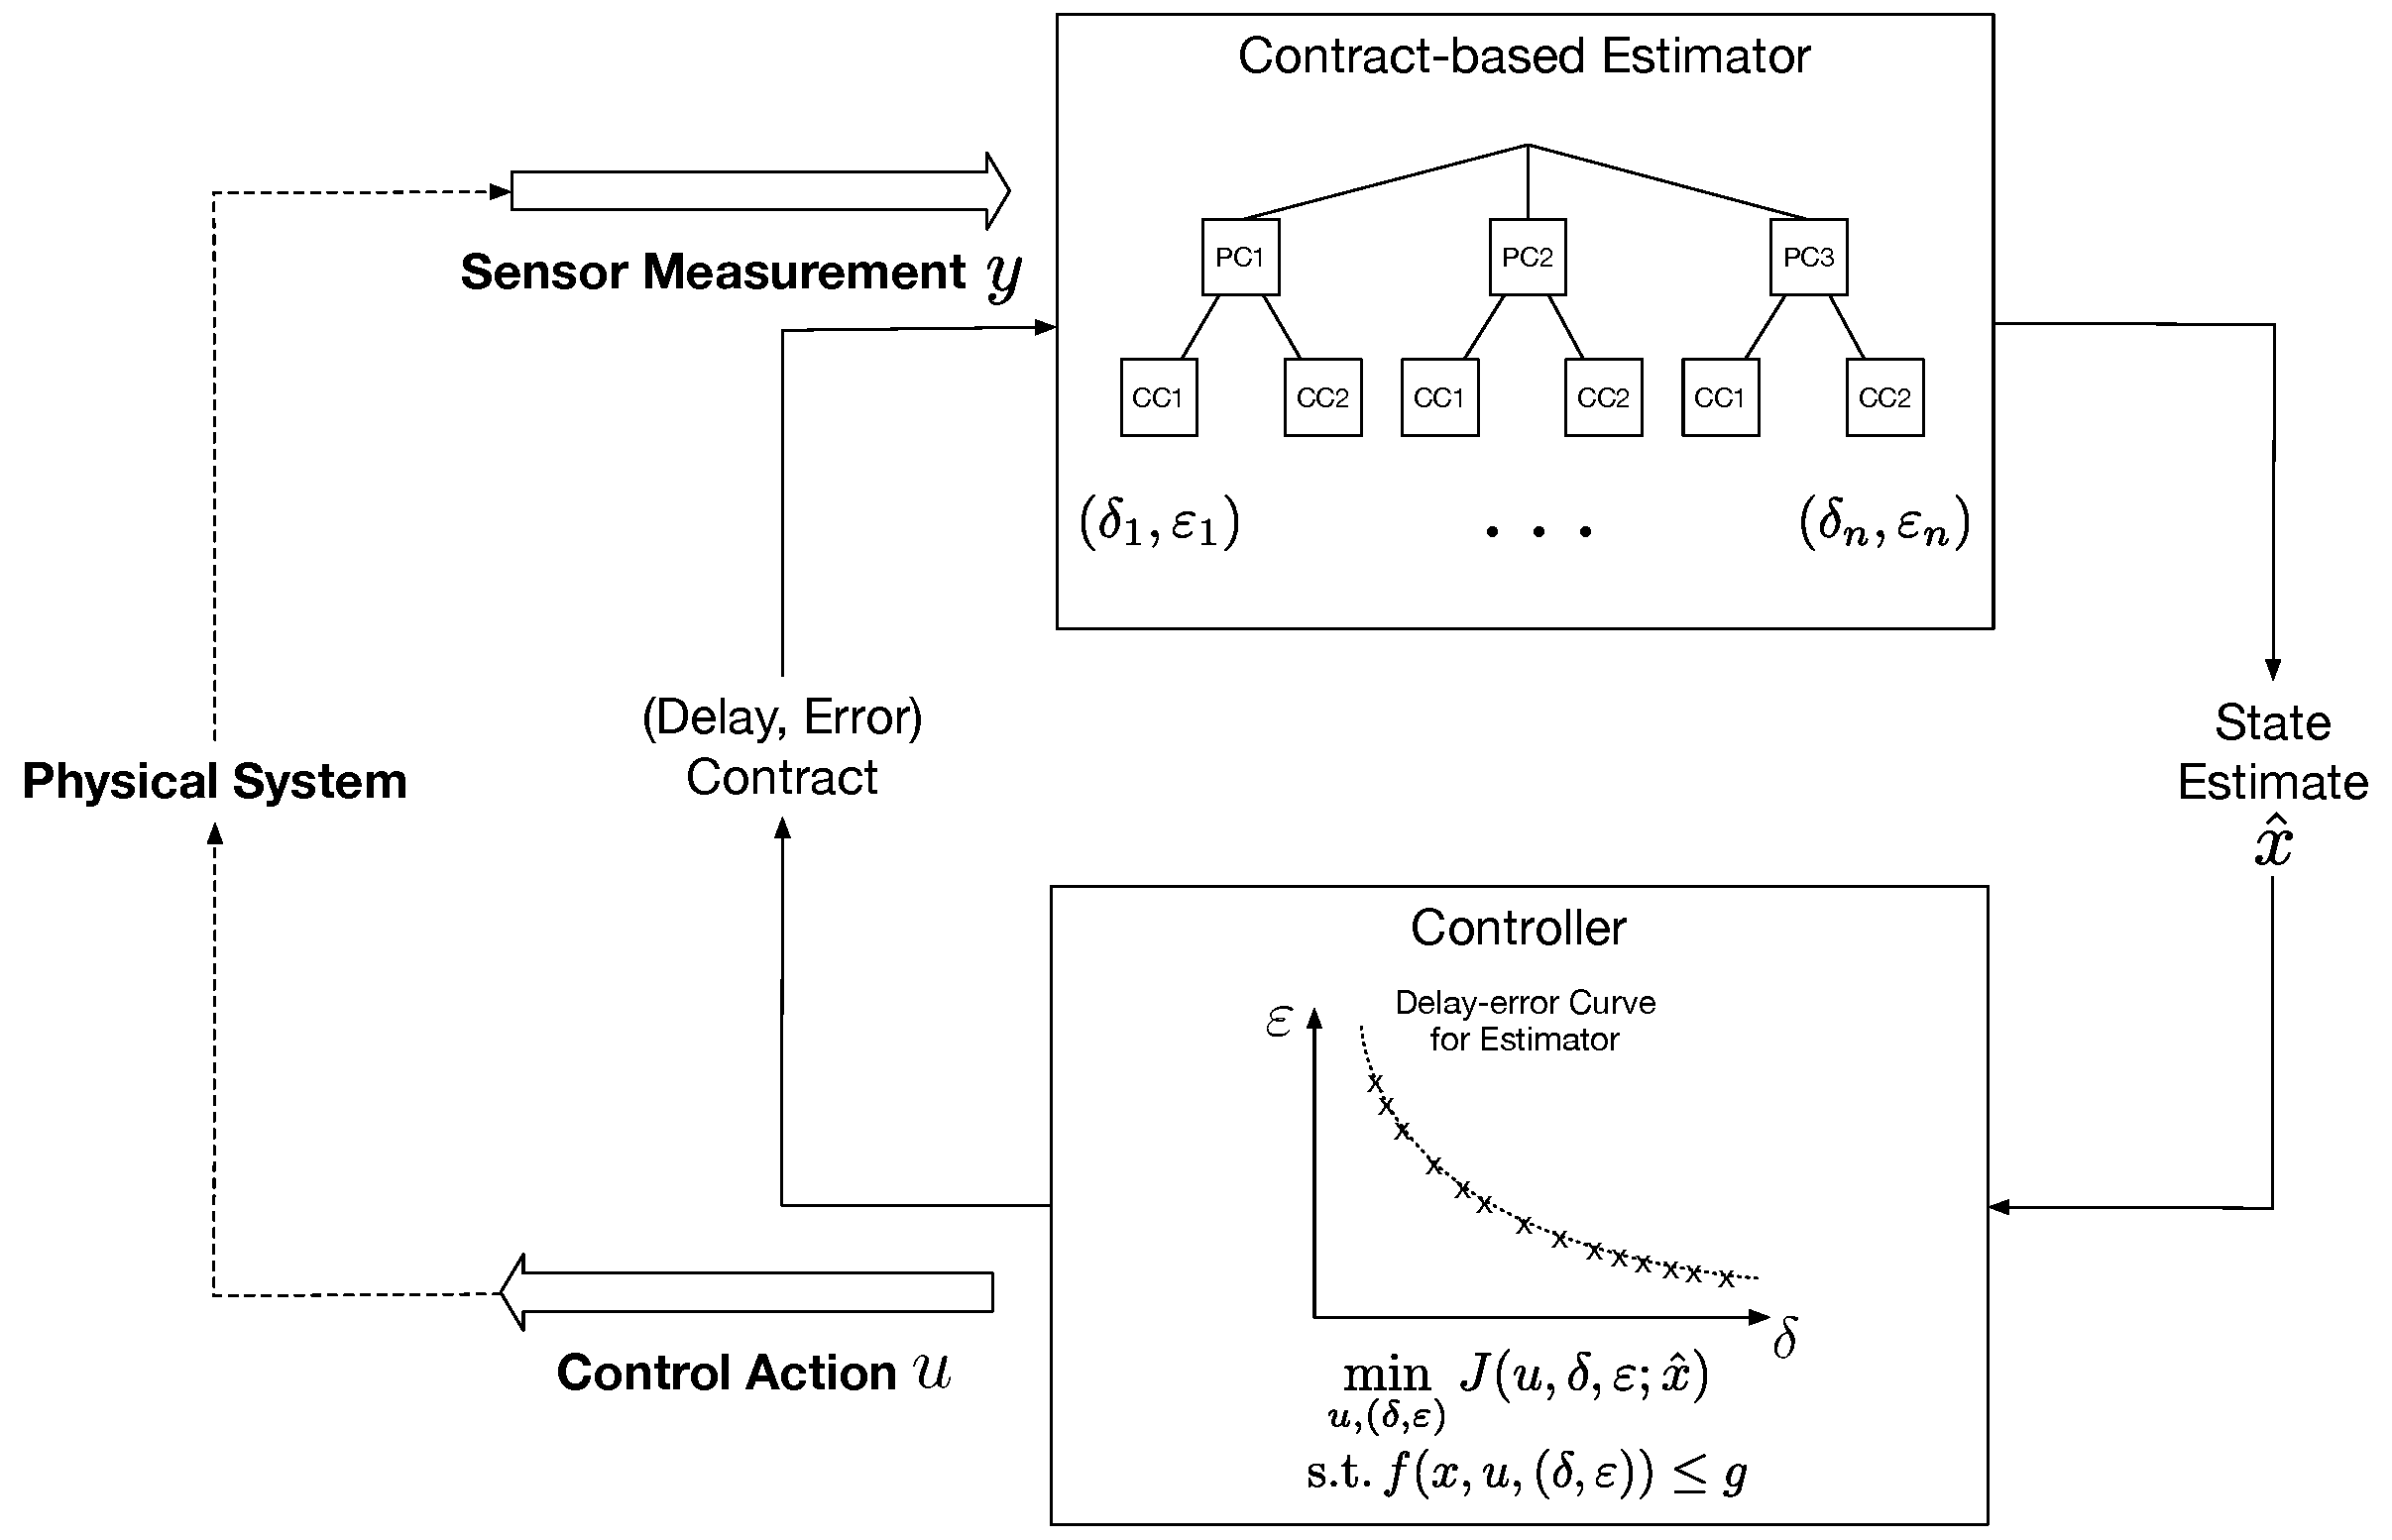
\includegraphics[width=0.49\textwidth]{figures/omnigraffle_figures/mid_level_figure2}
	\caption{Contract-based estimator and controller}
	\label{fig:fullcodesignedCE}
\end{figure}
\subsection{Contract based perception algorithms}

In order to maximize the efficiency of the computation and control system, a contract based perception algorithm can operate at different deadlines and provide a usable solution for the control algorithm to operate on. This flexible operation of the generally run-to-completion algorithms is achieved by composing the algorithm of functional blocks that have different computation times and result in different qualities of outputs. Note that this problem is different from that of composing multiple anytime algorithms together \cite{zilbersteinAImag}. Anytime algorithms \cite{boddy} have a well defined computation time versus quality tradeoff, but in our case we are composing together blocks that are individually run-to-completion and in most cases do not have a well defined intermediate measurable quality.

Figure \ref{fig:RT_bs} shows an example where an object recognition algorithm is composed of different functional blocks of varying computation time and result in a different accuracy when linked together to provide the functionality of an object recognition algorithm, e.g. the pixel classifier in the first stage could be a Gaussian Mixture Model with 2, 4, or 6 components, with more components providing better classification performance (over-fitting is ruled out by cross-validation) at the cost of more computation time. Functions with similar characteristics like example above, when profiled extensively offline and composed in the right order at run-time can be used to compose a contract time anytime perception and estimation algorithm. More details follow in section \ref{delayErrorCurve}.

%The output of the pixel classifier, which is a binary image, can then be filtered and connected into objects using a variety of filters and connected component methods. Finally the connected objects have to pass through a shape classifier to ensure that we detect only the object of interest.

%.... \textbf{<more details here>}.

%This composition of individual components can be represented as a decision tree where edges are blocks of code and nodes are their intermediate outputs/input to the next stage. An extensive profiling stage at design time helps assign distributions for execution times to the edges and distributions for output quality to paths along the tree. At run-time, this knowledge of execution times and output quality distributions can be used to generate a composition to realize a given criteria. An example of a criteria is to maximise the expected quality while meeting the given deadline with a high probability $\eta$.



%Given a decision tree with pre-profiled information about execution time distributions for edges and quality for paths, this optimization can be mapped to an integer programming problem for edge selection in the tree. This problem can be solved in a

%\textbf{<more details on the optimization here>}

\subsection{Interface between contract based perception and robust control}

For the control algorithm to be able to leverage the flexible nature of the contract based perception algorithm, it must have information about the computation time versus output quality trade-off that the contract based perception algorithm offers, but should not be exposed to too much detail or made dependent on how the trade-off is obtained. An interface that achieves this is obtained by simply representing the profiled behaviour of the contract based algorithm to varying deadlines, as points on a perception quality versus deadline ($\delta, \epsilon$) curve, e.g. in figure \ref{fig:eps_delta_toy}.
With this profiled curve available to the controller at runtime, the exchange of information between the contract based perception algorithm and the control algorithm consists of the controller assigning a deadline ($\delta$), or a contract to the perception algorithm with an expected bound on the quality ($\epsilon$) of its output. The perception algorithm then returns an output after internally deciding the composition to best meet the deadline and the expected quality requirement. While in many systems, assigning a contract for time and simultaneously expecting a minimum quality output may be an infeasible proposition, in this paper we only consider settings where neither the $\delta$ contract nor the $\epsilon$ bound are violated. This helps in formulating a control algorithm that provides mathematical guarantees on the feasibility of constraints for the safe operation and stability of the closed loop dynamic system as is covered in section \ref{robustMPC}.

\begin{figure}[t]
	\centering
	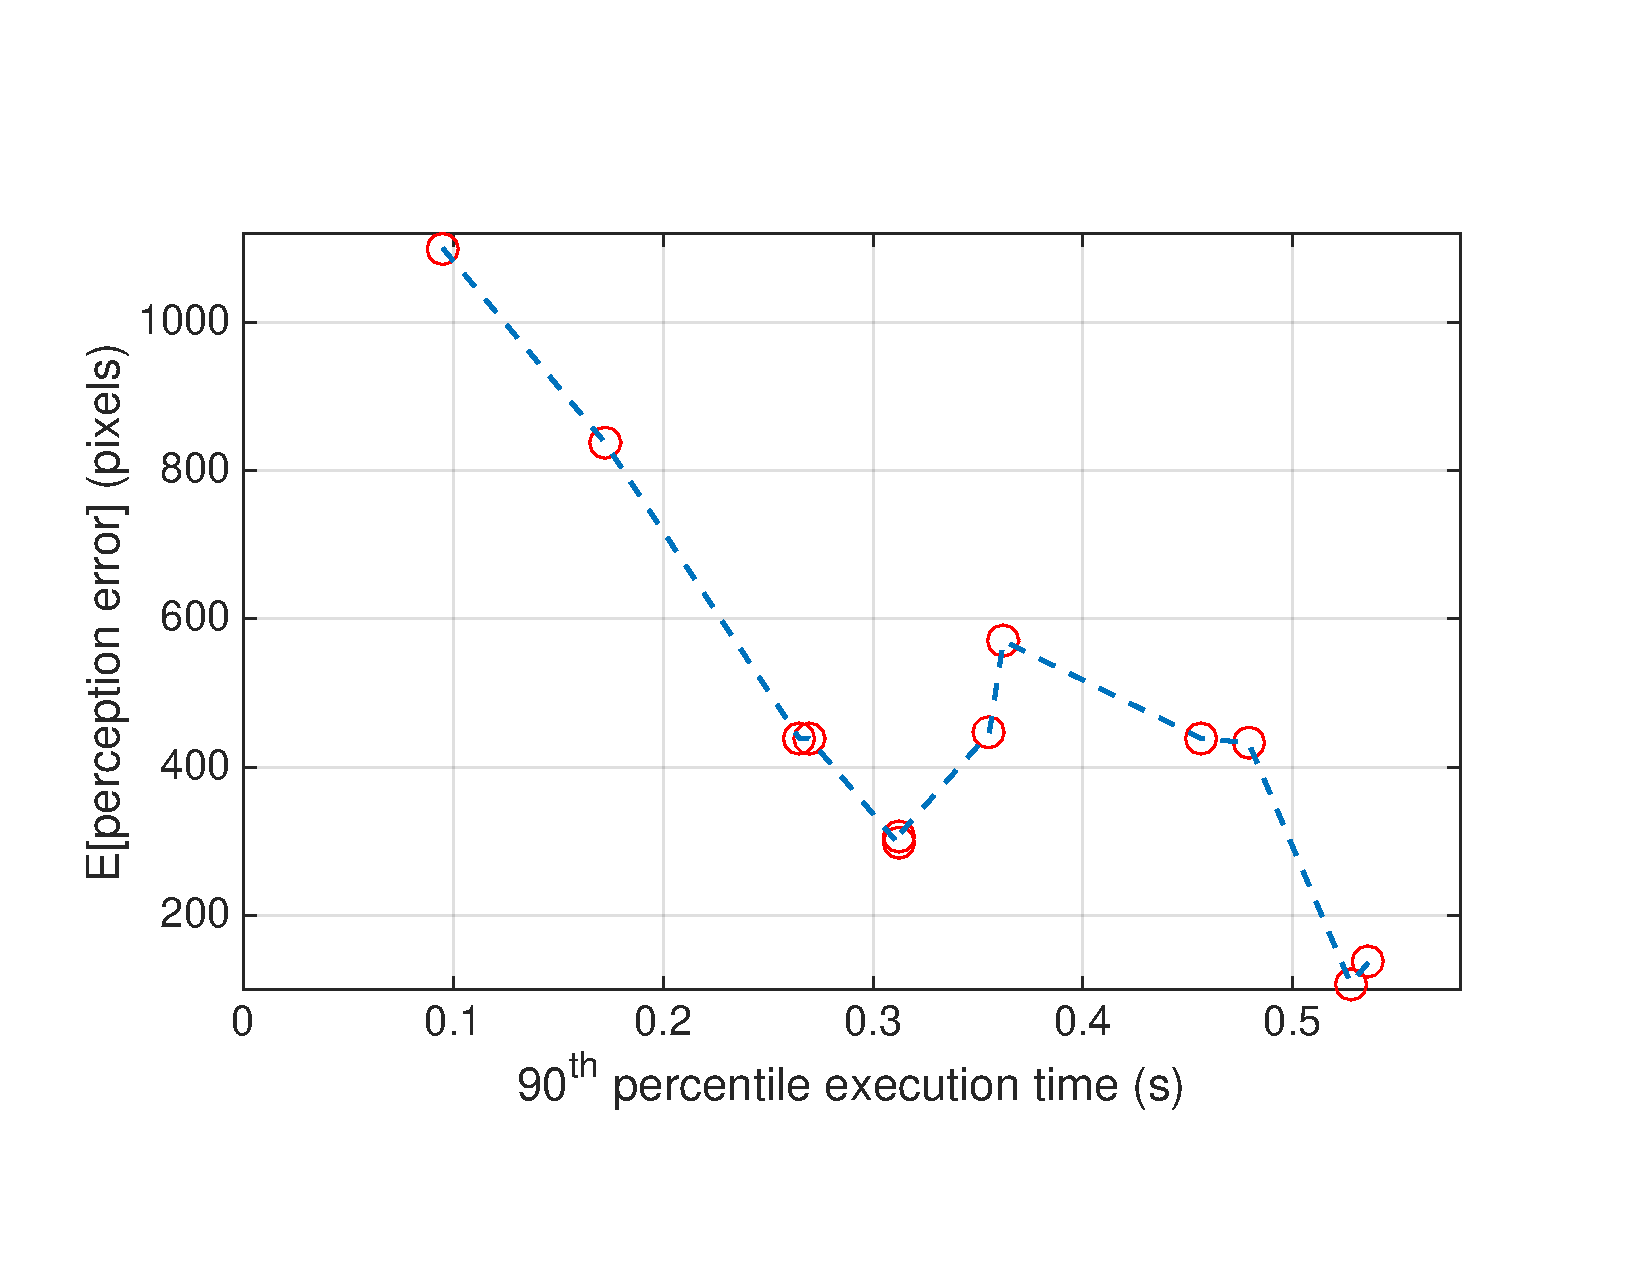
\includegraphics[width=0.49\textwidth]{figures/chainErrorDelay}
	\caption{Profiled perception versus computation time curve for an object detection algorithm run at different parameter settings.}
	\label{fig:eps_delta_toy}
\end{figure}

\subsection{Robust Control with contract based perception algorithm}

The control algorithm is designed to pick the best operating point for the estimator, or the right $\de$ contract to request the perception and estimation algorithm to meet. This is done based on the current state of the dynamic system to maximize a performance measure while being robust to the varying computation time, which shows up as a delay to the control algorithm, and the varying quality of output, which are varying estimation errors to the controller. In section \ref{robustMPC} we present a control algorithm that achieves this while also guaranteeing feasibility of system constraints the stability of the closed loop system.







	\section{Robust Control with Contract-Based Estimator}
\label{controlProblem}
In this section we present the mathematical formulation to model the controller and physical system from Fig. \ref{fig:codesignedCE}, and demonstrate how the controller can, in real-time, use knowledge of the estimator's error-delay curve to decrease computation delay and power in an error-aware fashion.

\section{Problem Formulation} \label{sec:formulation}

The control problem is as follows:

\begin{subequations}
\begin{align}
\text{Minimize } &l(x,u) \\
&\text{s.t.} \nonumber \\
\dot{x}&=f(x)+G(x)u \label{eq:NL_Plant} \\
x&\in X\\
u&\in U
\end{align}
\end{subequations}

Here, $x \in \mathbb{R}^{\dimX}$ and $u \in \mathbb{R}^{\dimU}$. A discrete-time, periodic, state-estimator provides access to a state estimate with estimation error

\begin{subequations}
\label{eq:NL_estimate}
\begin{align}
\hat{x}(t)&=x(t)+e(t) \\ 
\text{where, } e(t) &\in E
\end{align}
\end{subequations}

For sake of simplicity, for the rest of this paper, we assume $X$, $U$ and $E$ are hyper-rectangular, i.e. each dimension of $x$, $u$, $e$ has a fixed upper and lower limit, although the approach we use applies when these 3 sets are convex (bounded) polytopes of arbitrary form.

Given a subset $\Xc$ of a dynamical system's state space, and a horizon $T \geq 0$, the \emph{reachable set of the system from $\Xc$ in time $T$} is the set of states that the system visits, at time $T$ if it starts somewhere in $\Xc$.
Formally, $\RT{\Xc} \defeq \{y \in X \such \exists x_0 \in \Xc: x \text{ is a trajectory of the system, }x(0)=x_0, x(T)=y\}$.

\textbf{Notation}.
Given two subsets $A,B$ of $\Re^n$, define their \textit{Minkowski sum} to be $A\oplus B \defeq \{a+b \such a\in A, b\in B\}$.
Define their Pontryagin difference to be $A\ominus B = \{c \in \Re^n \such c+b \in A\; \forall b \in B\}$

	\section{Robust Model Predictive Control Solution}
\label{robustMPC}

In this section we give an overview of the \emph{Robust Adaptive Model Predictive Controller} (RAMPC) that we use in the contract-based setup of Fig.~\ref{fig:fullcodesignedCE}.
The mathematical details and derivations are available in the Appendix.
Experiments confirm that the following controller can be run in real-time, and uses a negligible amount of time to compute relative to the estimation delay $\sDelay$ (see Fig.~\ref{fig:senseActuate}).

\subsection{Solution overview}
Recall the operation of the contract-based control and estimation framework as presented in Section \ref{sec:codesign} and Fig.~\ref{fig:fullcodesignedCE}.
First, the estimator is profiled offline to obtain its delay-error curve, which we denote by $\Delta$.
The curve $\Delta$ represents a finite number of $\de$ contracts that the estimator can satisfy.
%Let $|\Delta|$ be the number of such contracts on the curve $\Delta$.
At every time step $k$, the controller receives a state estimate $\hat{\stPt}_k$ and uses it to compute two things:
first is the control input $\inpPt_{k}$ to be applied to the physical system at time $t_{a,k}$.
The second is the contract $(\sDelay_{k+1}, \sAccu_{k+1}) \in \Delta$ that will be requested from the estimator at the next step.
At $k+1$, the estimator provides an estimate with error at most $\sAccu_{k+1}$ and within delay $\sDelay_{k+1}$.
Finally, recall that \todo[inline]{Do we want to keep the $\infty$?}$J = \sum_{k=0}^{\infty}\left(\ell(\stPt_k,\inpPt_k)+ \alpha \pi(\sDelay_k)\right)$ combines tracking error and input power in the $\ell$ terms, and estimation power consumption in the $\pi$ terms.

The contract-based controller's task is to find a sequence of inputs $u_k \in \inpSet$ and of contracts $(\sDelay_k, \sAccu_k) \in \Delta$ such that the cost $J$ is minimized, and the state $\stPt_k$ is always in the set $\stSet$.
The challenge in finding the control inputs is that the controller does not have access to the real state $\stPt_k$, but only to an estimate $\hat{\stPt}_k$.
The norm of the error $e_k = \hat{\stPt}_k - \stPt_k$ is bounded by the contractual $\sAccu_k$, which varies at each time step.

Fix the \emph{prediction horizon} $N \geq 1$.
Assume that the current contract (under which the current estimate $\hat{\stPt}_k$ was obtained) is $\dek{k}$, and that the previously applied input is $\inpPt_{k-1}$.
To compute the new input value $\inpPt_{k}$ and next contract $\dek{k+1}$, the proposed \textbf{Robust Adaptive Model Predictive Control (RAMPC)} seeks to solve the following optimization problem which we denote by $\RAMPCProb{\Delta}{k}$:
\begin{eqnarray}
\label{eq:fullOptim}
&& \min_{\inpSig,\sttraj,\sDelayV,\sAccuV} J[0:N]
\\
= && \min_{\inpSig,\sttraj,\sDelayV,\sAccuV}\sum_{j=0}^{N}\left(\ell(\Nom \stPt_{k+j},\inpPt_{k+j})+\pi(\sDelay_k)\right)
\nonumber
\end{eqnarray}
I.e., RMPC needs to find the optimal length-$N$ input sequence  $\inpSig^* = (\inpPt_k^*,\ldots,\inpPt_{k+N}^*) \in \inpSet^N$, corresponding state sequence $\sttraj = (\stPt_k,\ldots,\stPt_{k+N}) \in \stSet^N$, delay sequence $\sDelayV = (\sDelay_k,\ldots,\sDelay_{k+N})$ and error sequence $\sAccuV = (\sAccu_k,\ldots,\sAccu_{k+N})$ such that $\dek{k} \in \Delta$, which minimize the $N$-step cost $J[0:N]$.
In the remainder of this section we discuss how to make this problem tractable.
As in regular MPC, once a solution $\inpSig^*$ is found, only the \emph{first} input value $u_k^*$ is applied to the physical system, thus yielding the next state $\stPt_{k+1}$ as per \eqref{eq:disc-dynamics}.
At the next time step $k+1$, RAMPC sets up the new optimization $\RAMPCProb{\Delta}{k+1}$ and solves it again.

To make this problem tractable, we first assume that the mode is fixed throughout the $N$-step horizon, i.e. $\dek{k+j} = \de$ for all $1 \leq j \leq N$.
Thus for every value $\de$ in $\Delta$, we can setup a different problem \eqref{eq:fullOptim}, which we denote by $\RAMPCProb{\de}{k}$, and solve it.
Let $J_{\de}^*$ be the corresponding optimum.
The solution with the smallest objective function value yields the input value $\inpPt^*_k$ to be applied.

\begin{figure}[t]
\centering
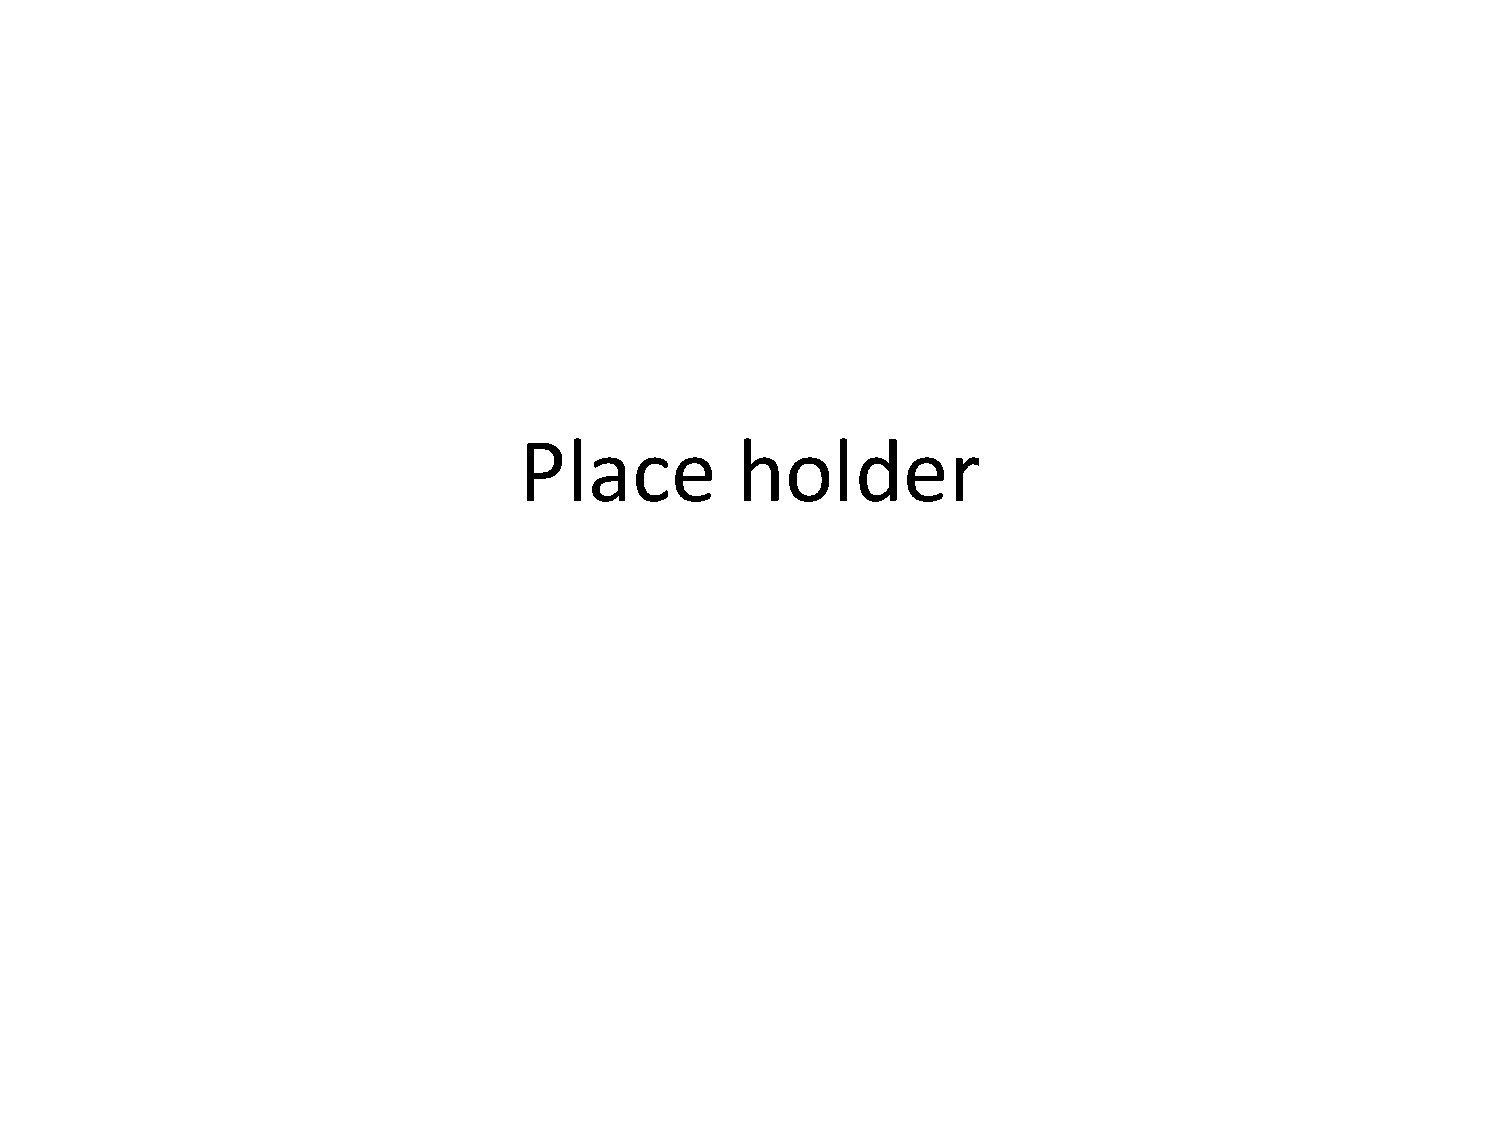
\includegraphics[width=0.7\linewidth]{figures/placeHolder}
\caption{RAMPC algorithm: at every step, the constraint set is reduced to guarantee satisfaction of the original constraints.}
\label{fig:placeHolder}
\end{figure}

Because RAMPC only has access to the state estimate, we extend the RMPC approach in \cite{richardsetal05rmp, chiscietal01swp}.
Namely, the problem is solved for the \emph{nominal dynamics} which assume zero process and observation noise ($w_{k+j} = 0)$ and zero estimation error ($\hat{\stPt}_{k+j}=\stPt_{k+j}$) over the prediction horizon.
Let $\Nom \stPt$ be the state of the system under nominal conditions.
To compensate for the use of nominal dynamics, RMPC replaces the constraint $(\Nom\stPt_{k+j},\inpPt_{k-1+j}) \in \stSet \times \inpSet \defeq \ZSet$ 
by $(\Nom \stPt_{k+j},\inpPt_{k+j}) \in \stSet_{k+j} \times \inpSet_{k+j} \defeq \Zc_{k+j}$,
where $\Zc_{k+j} \subset \ZSet$ is $\ZSet$ `shrunk' by an amount corresponding to $\sAccu_k$, as explained in the Appendix.
Intuitively, by forcing $(\Nom\stPt_{k+j},\inpPt_{k-1+j})$ to lie in the reduced set $\ZSet_{k+j}$, the bounded estimation error and process noise are guaranteed not to cause the true state and input to exit the constraint sets $\stSet$ and $\inpSet$.

Algorithm \ref{algo:RMPC-algo} summarizes the RAMPC algorithm.
\begin{algorithm}
	\begin{algorithmic}[1]
		\State $\dek{0}$ and $u_{-1}$ specified by designer
		\State Apply $u_{-1}$
		\For{$k=0,1,\dots$}
		\State Estimate $\hat{\stPt}_{k}$ with guarantee $\left(\sDelay_k, \sAccu_k\right)$
		\For{each $\left( \sDelay,\sAccu \right) \in \Delta$}
		\State $J_{\sDelay,\sAccu}^* \leftarrow $ Solve $\RAMPCProb{\de}{k}$		
		\EndFor
		\State $( \sDelay^{*}, \sAccu^{*}, u_{k | k}^{*} ) \gets \argmin_{\sDelay,\sAccu} J_{\de}^*$
		%\State Wait until $t_{a,k}$
		\State Apply control input $u_{k} = u_{k | k}^{*}$ and estimation mode $\dek{k+1} = \left( \sDelay^{*}, \sAccu^{*} \right)$
		\EndFor
	\end{algorithmic} 
	
	\caption{Robust Adaptive MPC algorithm with Anytime Estimation.}
	\label{algo:RMPC-algo}
\end{algorithm}

We prove the following result in the Appendix:
\begin{thm}%[Robust Feasibility of RMPC with Anytime Estimation]
	\label{thm:robust-feasible-anytime-RMPC}
	If at the initial time step there exists a contract value $\de \in \Delta$, 
	an initial state estimate $\hat{\stPt}_0 \in \stSet$,
	and an input value $\inpPt_{-1} \in \inpSet$,
	such that $\RAMPCProb{\de}{0}$
	is feasible then the system (\ref{eq:disc-dynamics}) controlled by
	Alg.~\ref{algo:RMPC-algo} and subjected to disturbances constrained
	by $w_k \in \Wc$ robustly satisfies the state constraint $\stPt \in \stSet$
	and the control input constraint $\inpPt \in \inpSet$,
	and all subsequent iterations of the algorithm are feasible.
\end{thm}





	\section{Contract based perception algorithms}
\label{delayErrorCurve}

In Section \ref{sec:codesign}, we postulated the existence of an Estimation Error vs Computation Delay ($\delta,\epsilon$) curve. % (the `error-delay curve').
This curve is used at every time step by the controller to determine the operating point $(\delta,\epsilon)$ for the next time step.
In this section we demonstrate in detail how such a curve may be obtained for particular applications and how points along the curve are realized at runtime by the contract based perception algorithms.

\subsection{Profiling and composing an anytime contract based perception algorithm}

Recall, in section \ref{sec:codesign} we briefly discuss how a contract based perception tool chain can be obtained by composing different version of the individual run-to-completion algorithms used in the perception algorithm. The first stage towards this is to identify the different individual components of the perception tool chain and identifying how to realize different computation time and accuracy versions of them. We refer to these different realizations  knobs for the perception algorithm, and the control knobs may be as simple as changing the number of iterations in a loop \cite{greenMS} or finding alternate implementations with different resultant execution times and performance for the same functionality. As a running example in this section to illustrate our methods, we consider a perception tool chain for object recognition from camera images. An overview of the flow and individual components of the tool chain is shown in figure \ref{}.

This tool chain takes in a video stream and tracks an Object Of Interest (OOI) across the frames. The first stage of it is a pixel classifier that assigns to each pixel of the image (after potential pre-processing) the probability of its being a pixel of interest, i.e., of belonging to an OOI or being a part of the background. A binary image is then obtained which assigns the value 1 to pixels of interest, and 0 to all others. A knob here in the pixel classification stage is to realize different computation time and performance profiles, is the complexity of the probabilistic model used to detect whether a pixel belongs to the object of interest. The knob in this case is whether we choose a Gaussian Mixture Model (GMM) with fewer components, which would be faster but less accurate, versus a GMM with more components which will take more computation time but provide better classification performance. Knobs where we over fit the training data are removed by cross-validation stage as is standard. Next, filtering and a Connected Components (CC) algorithm is run on the binary image to get rid of noise in the classification process and segment its 1-valued pixels into disconnected objects. A shape classifier is then run on each object to determine whether it is an object of interest or not.
% the pixel classifier is a Gaussian Mixture Model (GMMs), whose knob is the number of Gaussians in the mixture.
In our implementation for the object detector that we use as the illustrative example here, the pixel classifier is a GMM based classifers with the number of knobs being the number of components in the GMM as discussed above. The filtering and connected components algorithm are lumped into one stage and have a two-valued knob to choose between a 4-connected and 8-connected component implementation. The shape classifier is also a GMM, but the knob for it is the number of shape features resulting in Gaussians in different dimensions being fit, and hence resulting in different computation time and classification accuracy.
% The number of Gaussian components for the shape classifier is fixed since we know in advance the number of objects in the training and test sets.
In the given setting the number of knob settings for the entire chain is $K$ = (\#Gaussians for pixel classifier, \#neighbors for CC, \#features for shape classifier), and has a total of $3 \times 2 \times 2 = 12$ values.

Note that for any given algorithm in the chain, the relation between knob value and quality of output is not necessarily monotonic. The pixel and shape classifiers are machine learning algorithms that need to be trained on a training set before being used and like all machine learning algorithms, their output quality for a given knob setting will depend on the actual data set.
The same is a fortiori true of the quality of the output of the entire chain. This is also reflected in figure \ref{}, where the solid line shows the mean perception error (measured as the 2-norm of the x,y co-ordinates of the centroid of the object and the estimated centroid from the object recognition algorithm) and the $90^{th}$ percentile execution time for the different knob settings. For the object detection algorithm we use for illustration in this section, we use images (of size 1200x1600 pixels) of red barrels at different distances and in different backgrounds.

The second stage to composing a contract based perception algorithm is to again use the training data to profile all the possible combinations of knobs through an extensive training and validation phase. This profiling gives us: a) Not only the output quality (or accuracy) of the perception tool chain under consideration, but also b) probability distributions for execution times for the stages of the perception tool chain under different knob settings. Note, since intermediate qualities are not easily measurable or assignable for some of the blocks of the tool chain (e.g. Connected Components) and for many other algorithms in general, we assign quality (or accuracy) distributions to the realizations of the complete tool chain by composing together different knob settings. Note, this profiling stage is done at offline at design time and provides us information that we use at runtime.

\subsection{Decision tree based run-time execution of the contract based perception algorithm}

After the contract based perception algorithm has been composed and the execution time distributions of its individual components and the quality distributions from composing together various knob settings have been profiled, we can represent the offline profiled algorithm as a decision tree as shown in figure \ref{} for run-time decisions. This decision tree based representation, where edges represent individual functions for different knobs, e.g. GMM based pixel classifier with 3 components, edges have assigned to them the execution time distributions of the functions they represent. Also, paths from the top of the tree to a leaf represent one particular realization of the tool chain and have assigned to them distributions for accuracy of the algorithm. The decision of selecting which knob setting to use for a particular stage for a given criteria can now be posed as an optimization problem for edge selection in the decision tree. For example, consider the case where we want to minimize the perception error while meeting a time deadline with a given high probability, the problem can be written as a constrained minimum cost path selection problem where timing information of the edges and quality information about paths can easily be encoded. This problem can be re-solved after each stage is executed with a recalculated time remaining and smaller decision tree structure for subsequent remaining stages. This allows the algorithm the flexibility to re-optimize its execution path (or knob settings) after obtaining updated information on time consumed in the past stages. For problems that do not have an excessively large number of knobs, such an optimization can be solved very quickly.

This decision tree based approach is also the equivalent of selecting different versions of tasks (knobs for stages) and scheduling them in sequential order to best perform the object recognition task while maximizing utilization (or estimation accuracy) and meeting the given time contract or deadline with a high probability. Figure \ref{} shows the different task versions for each knob in the different stages and the resulting schedule based on the knob settings for the stages. The offline profiling allows us to set the knobs such that we can achieve a feasible schedule for the given deadline, $\delta$ while maximizing the utility, or the expected accuracy of the perception algorithm.

\todo[inline]{Add T1+B1+G1 less than delta etc to both of the schedules to show time consumed and the feasibility of the schedule. Otherwise delta doesn't look very relevant for this fig}

\begin{figure}[htbp]
  \centering
  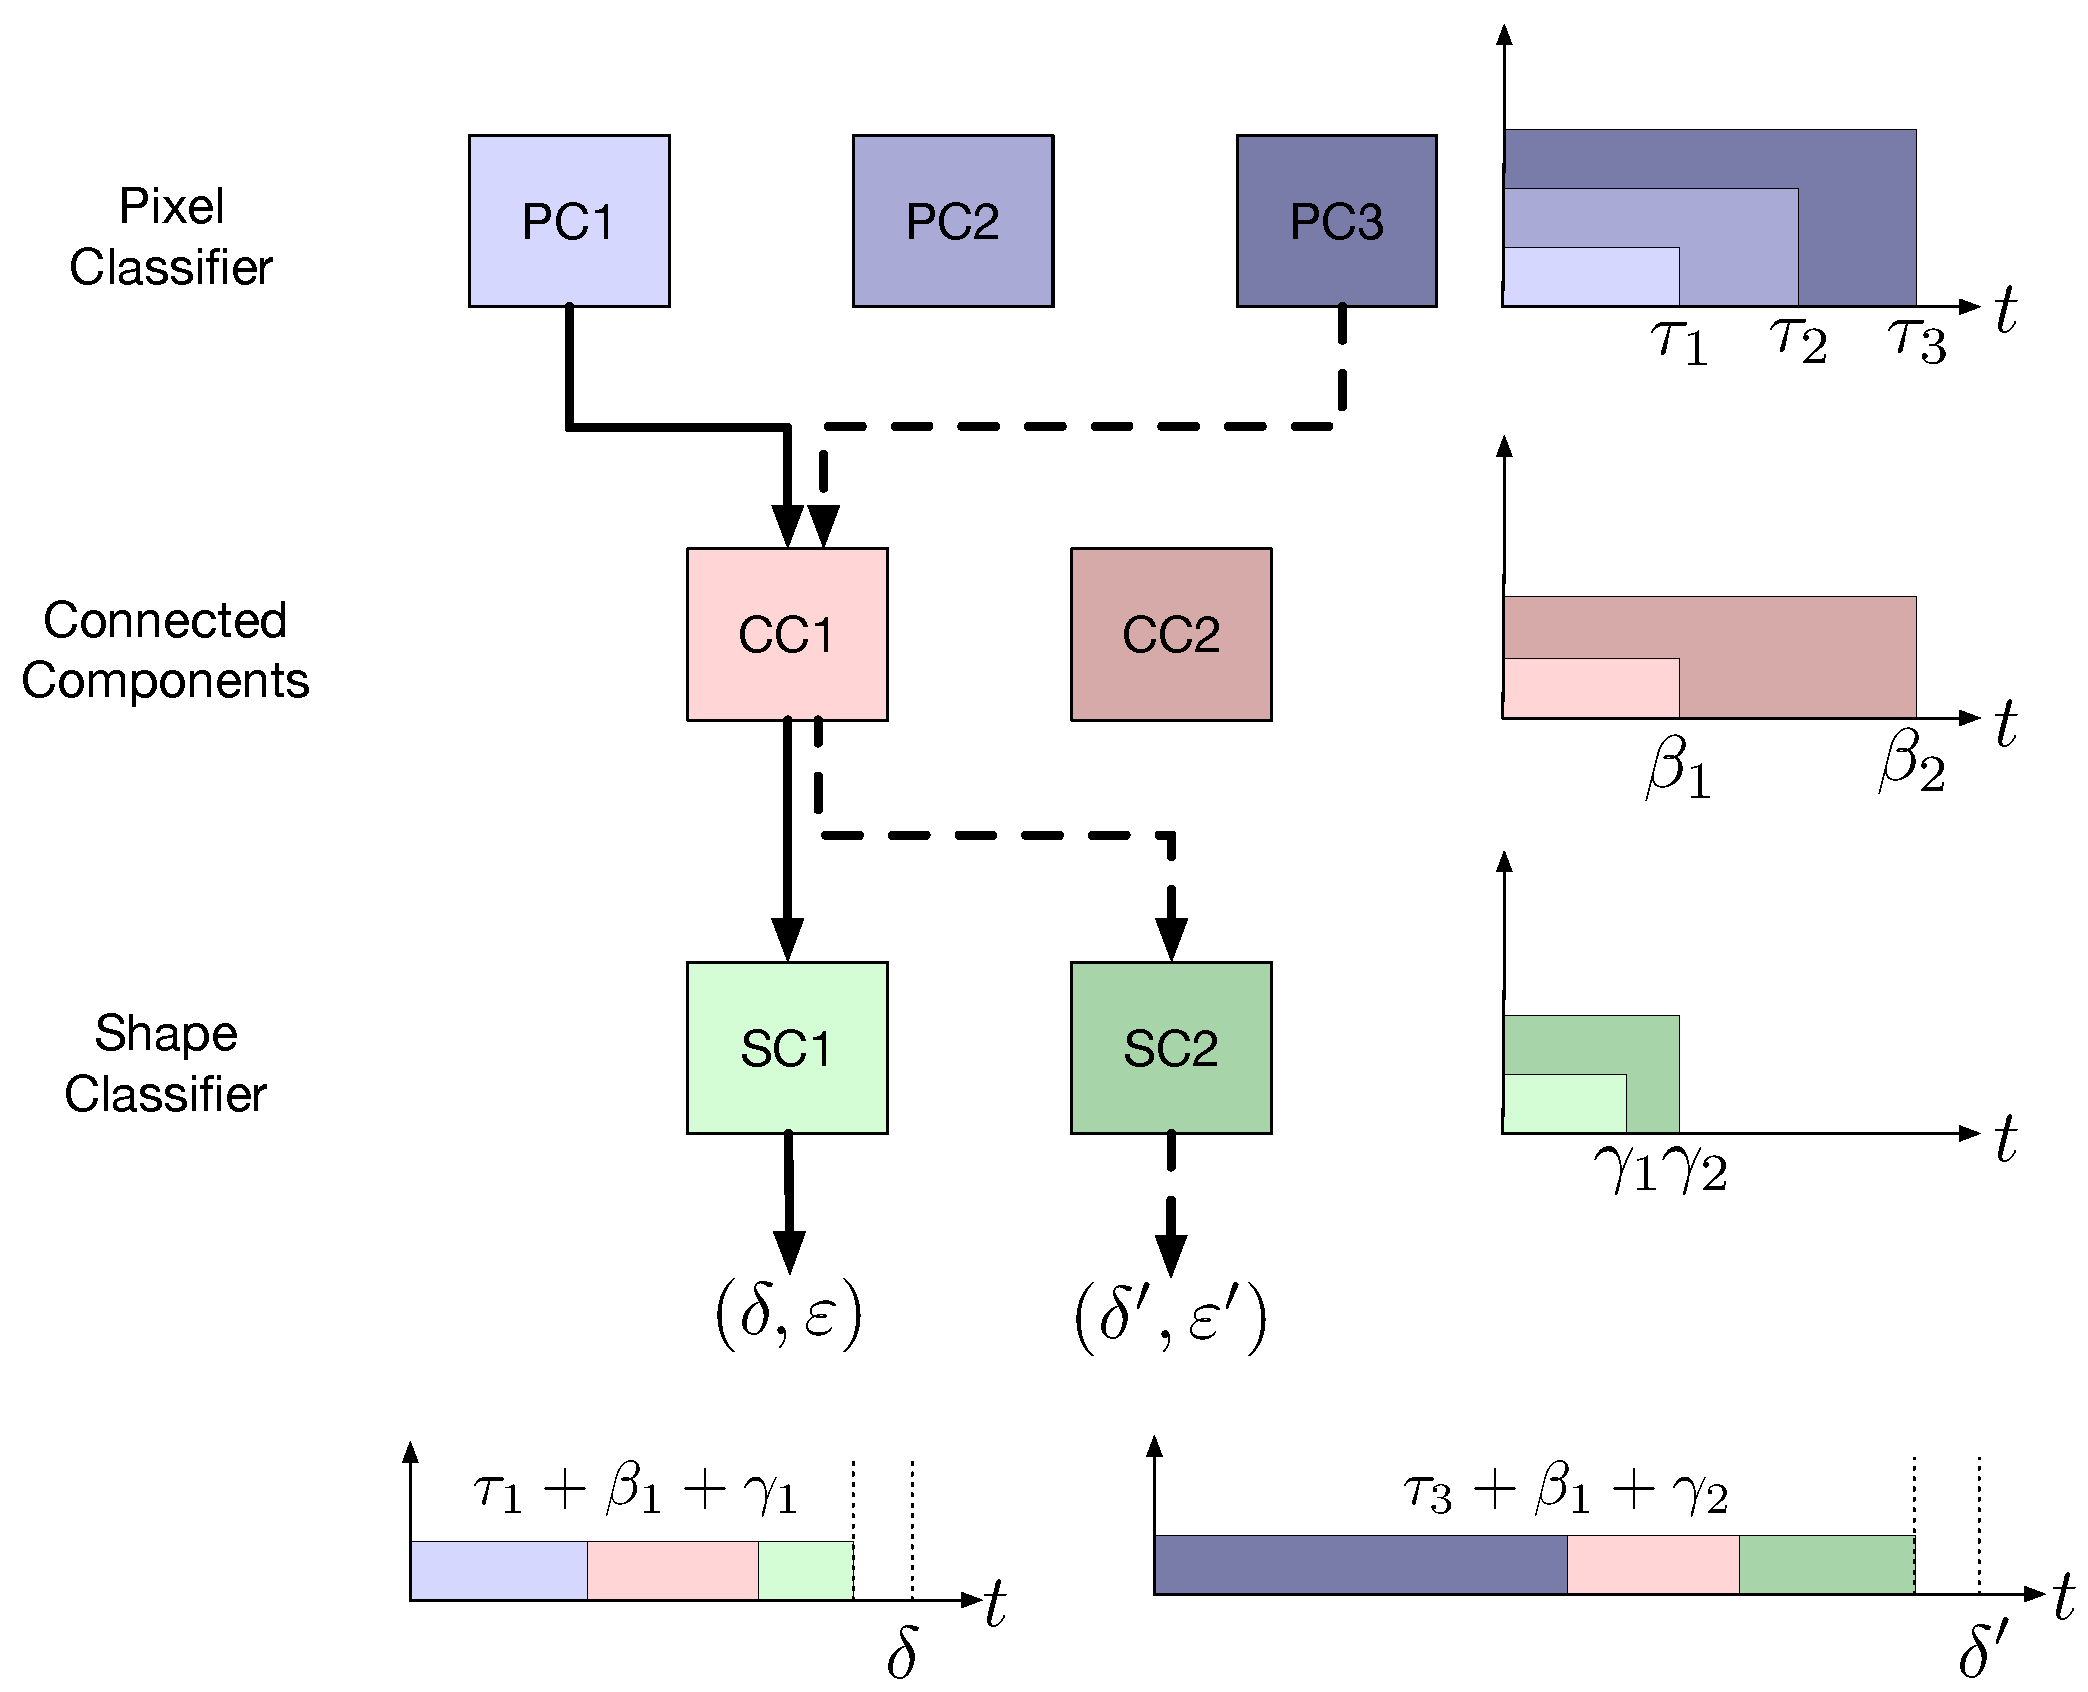
\includegraphics[width=0.9\columnwidth]{figures/omnigraffle_figures/real_time_figure}
  \caption{Illustration of the various components used to compose the contract based perception algorithm and their representation as real-time tasks. For a given deadline ($\delta$), knob settings are chosen at run-time resulting a feasible schedule to execute these sequential components, or tasks. The figure how choosing different knob settings for different deadlines result in different schedules.}
\end{figure}




%Specifically, we consider two different visual perception tool chains, where each tool of the chain has a knob that tunes its performance.%
%These knobs can be used to profile the tool chain and obtain its error-delay curve on particular platforms.
%Because power consumption is correlated to computation time, the error-delay curve can also be viewed as an error-power curve.
%The power consumption of the estimator task can be included in the control cost function using the $\alpha$ term of Eq.??.
%Thus, the controller can save power by selecting operating modes $(\delta,\epsilon)$ that achieve the control objectives at a lower energy cost.



% subsection
\subsection{Visual Odometry}

Another algorithm we consider is the Semi-Direct Monocular Visual Odometry (SVO)\cite{forster2014svo} which is used for estimating the position and orientation of the hexrotor using an onboard downward facing camera (see section \ref{sec:experiments}).
The visual odometry algorithm detects corners in an image and tracks them across video frames to perform self-localization of a moving robot.
These estimates are used in the closed loop control system that flies the hexrotor, hence it is important for the visual odometry to run at or faster than frame rate in order to provide a timely state estimate to the control algorithm
The number $\#C$ and quality of corners detected in a frame directly affects the runtime of the corner detector and the resulting quality of the state estimate. Generally speaking, detecting more corners requires a longer runtime, and results in better self-localization as long as we are analysing a feature rich scene, i.e., \emph{assuming acceptable quality of the detected corners}. Thus the number $\#C$ of corners is a knob which can be varied to obtain an error-delay curve for self-localization with the visual odometry algorithm.
If the scene is not rich enough in features, and a sizeable fraction of the $\#C$ corners are of poor quality (i.e., unstable or hard to track across frames), then we can expect the self-localization error to actually increase as the poor quality of the unstable corners detected adds noise to the visual odometry estimates.

Fig.~\ref{fig:svo_err_delay} shows the error-delay curve of self-localization error using the SVO.
The curve was obtained on an Odroid-U3 [??], which is the same processor as the one used on the hexrotor for on-board computation.
For each value of the knob $\#C$ (i.e., each requested number of corners), we ran the visual odometry algorithm on a video sequence recorded by the downward facing camera on the hexrotor while flying certain pre-set patterns.
Ground truth for computing the self-localization error was obtained using a Vicon motion capture system which provides position estimates with better than millimeter level precision.
As we repeat each flight several times, this results in a distribution of $(\delta,\epsilon)$ values for each value of $\#C$.
We retained the $90^{th}$ percentile values for $\delta$ and $\epsilon$, since these are used as worst-case estimates by the controller of Section \ref{controlProblem}.
It can be seen that a larger number of requested corners produces a smaller estimation error and longer runtime.
Starting at 250 corners, the error increases, however.
We hypothesize this is due to the decreasing quality of the corners being returned by the corner detection algorithm.
\begin{figure}[t]
\centering
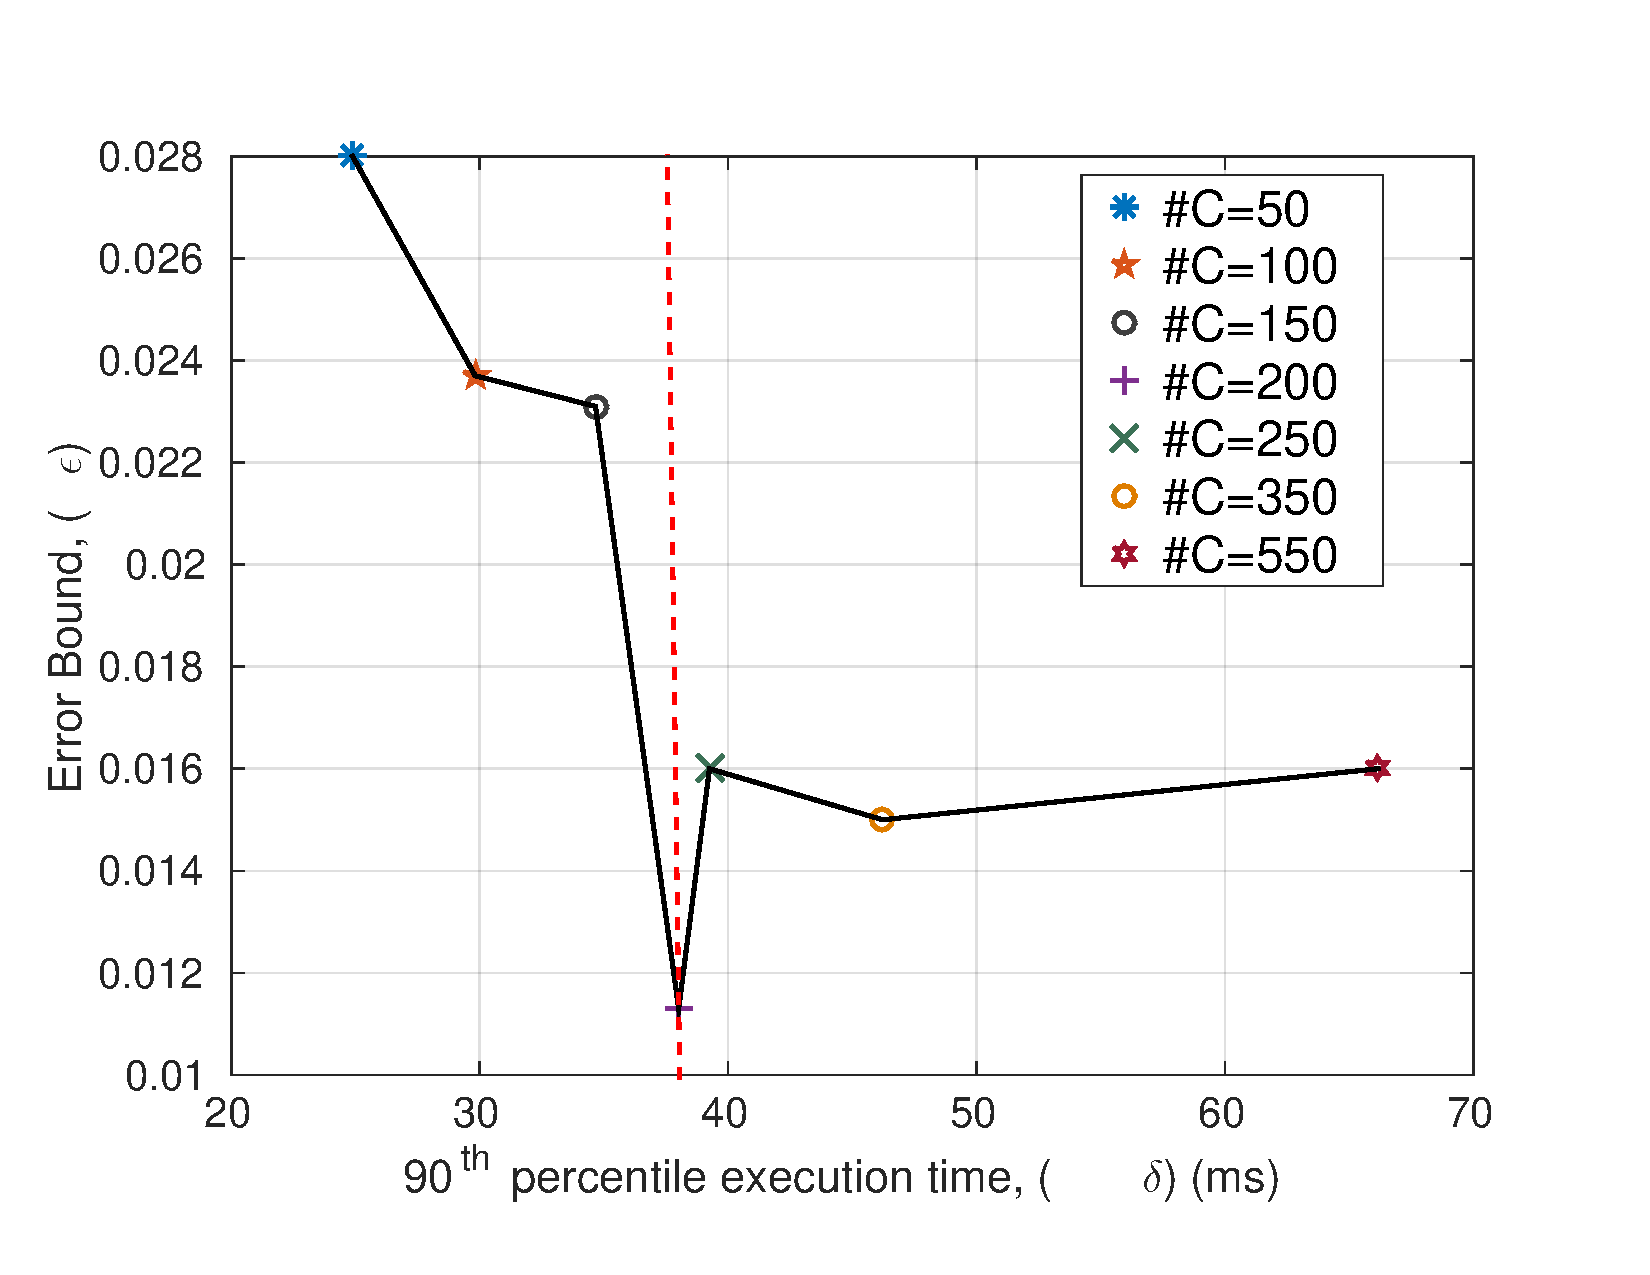
\includegraphics[width=0.9\columnwidth]{figures/errVsTime}
\caption{Error-delay curve for the SVO algorithm running on the Odroid-U3 - ?? Label where we stop choosing delays}
\label{fig:svo_error_delay}
\end{figure}

Fig.~\ref{fig:svoErrVsPower} shows the power consumption vs estimation error, which correlates well with Fig.~\ref{fig:svo_error_delay}.
\begin{figure}[t]
	\centering
	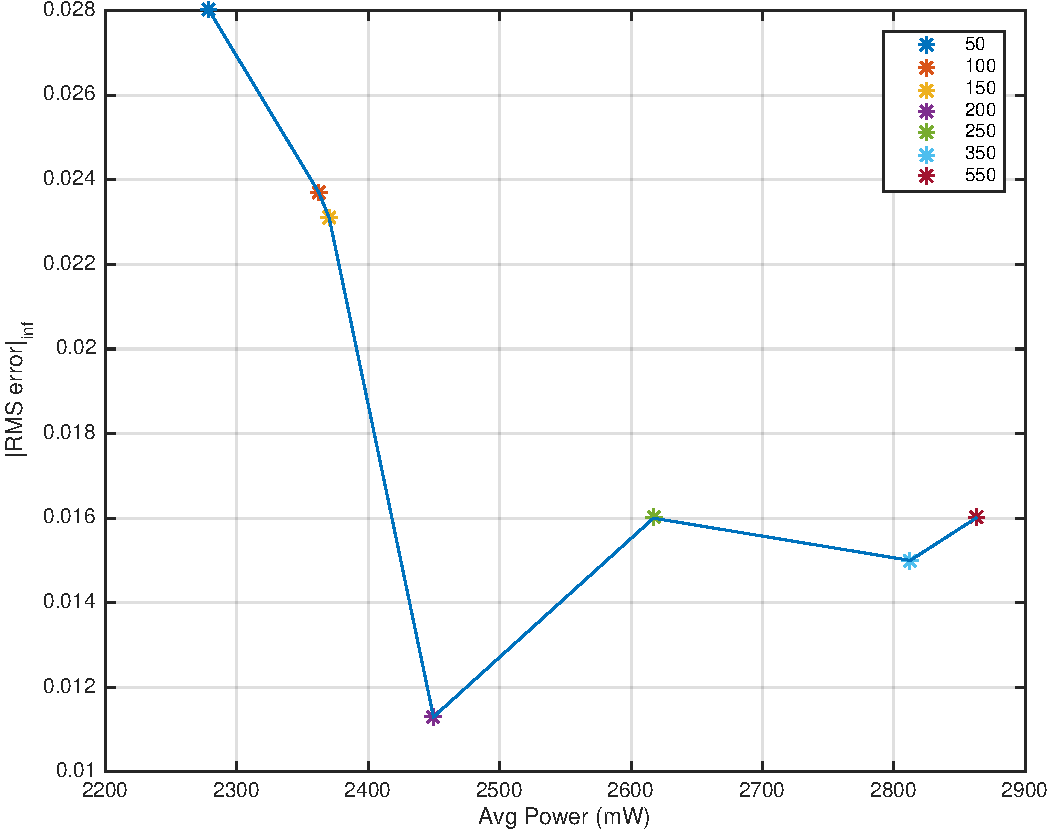
\includegraphics[width=0.9\columnwidth]{figures/errVsPower}
	\caption{Error vs power curve for the SVO algorithm running on the Odroid U3}
	\label{fig:svoErrVsPower}
\end{figure}

% subsection
%

\subsection{A contract time object recognition tool chain}

Our second example is a more complete perception tool chain shown in Fig.~\ref{fig:chain}.
\begin{figure}[t]
	\centering
	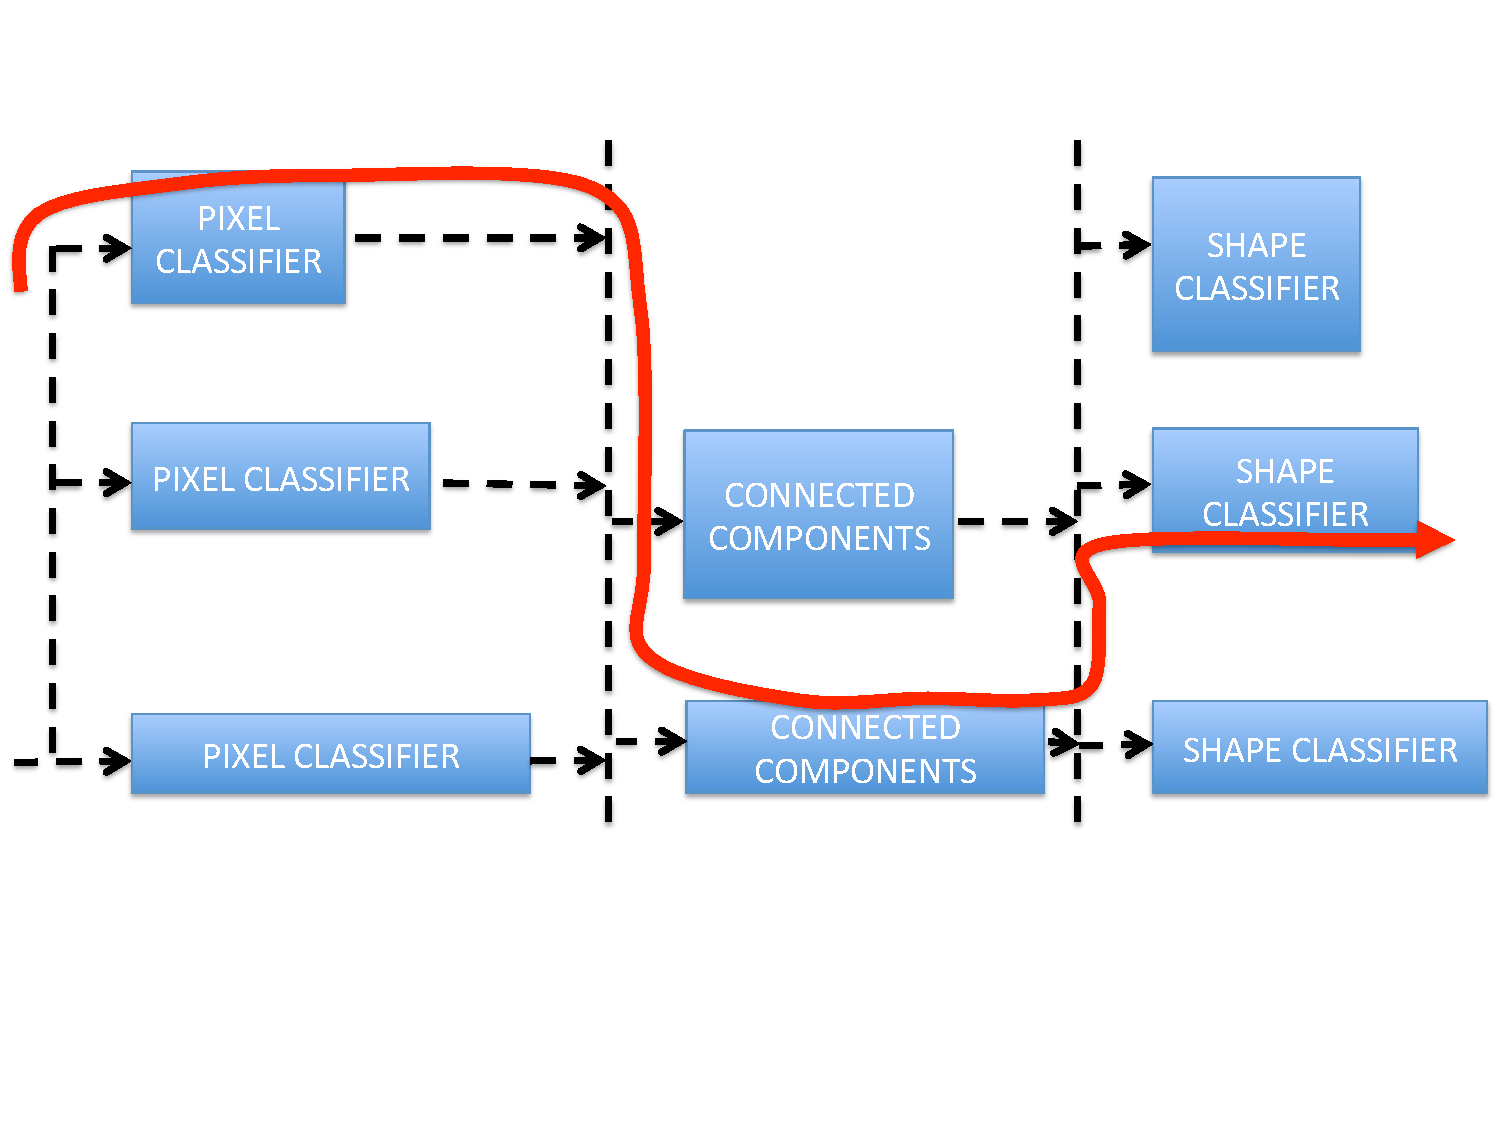
\includegraphics[width=0.7\linewidth]{figures/chain}
	\caption{Visual perception toolchain for object detection. The height of a block indicates output error, while width indicates runtime. The red path indicates one particular execution path which trades error for runtime at each stage.}
	\label{fig:chain}
\end{figure}
The tool chain takes in a video stream and tracks an Object Of Interest (OOI) across the frames.
The pixel classifier assigns to each pixel of the image (after potential pre-processing) the probability of its being a pixel of interest, i.e., of belonging to an OOI. 
A binary image is then obtained which assigns the value 1 to pixels of interest, and 0 to all others. 
A Connected Components (CC) algorithm is run on the binary image to segment its 1-valued pixels into disconnected objects.
A shape classifier is then run on each object to determine whether it is an object of interest or not.
The pixel and shape classifiers are machine learning algorithms that need to be trained on a training set before being used.
In our implementation of this chain, the specific algorithms and their knobs are as follows:
the pixel classifier is a Gaussian Mixture Model (GMMs), whose knob is the number of Gaussians in the mixture.
The connected components algorithm has a two-valued knob to choose between a 4-connected and 8-connected component implementation.
The shape classifier is also a GMM, but the knob for it is the number of shape features.
The number of Gaussian components for the shape classifier is fixed since we know in advance the number of objects in the training and test sets.
Thus the knob for the entire chain is $K$ = (\#Gaussians for pixel classifier, \#neighbors for CC, \#features for shape classifier), and has a total of $3 \times 2 \times 2 = 12$ values.
Note that for any given algorithm in the chain, the relation between knob value and quality of output is not necessarily monotonic. 
Like all machine learning algorithms, it will depend on the actual data set.
The same is a fortiori true of the quality of the output of the entire chain.

Fig.~\ref{fig:chainErrorDelay} shows the \emph{perception error}-delay curve for the object detection chain.
The perception error is the difference between the estimated centroid of the OOI and the true centroid of the OOI.
If the chain fails at finding the object in the frame, we assign that frame a constant error drawn from the errors found on other frames.
Each point on the curve was obtained by training the tool chain with the associated knob value, and then running the trained tool chain on the test set to obtain the $(\delta,\epsilon)$ values.
The plotted error value is the average error over all images in the test set.
The fact that the error \emph{increases} in some points despite increasing computation time can be explained by the remark made earlier: namely that the effect of a knob value is not necessarily monotonic on quality.
Moreover, the effect of a change to one algorithm of the chain might outweigh changes to other algorithms.
This makes profiling the end-to-end tool chain all the more important.
Thus, online, the controller can ignore the modes that show a degraded performance despite a higher energy cost.

This curve can then be turned into an estimate error-delay curve by incorporating it into an estimation algorithm.
\begin{figure}[t]
	\centering
	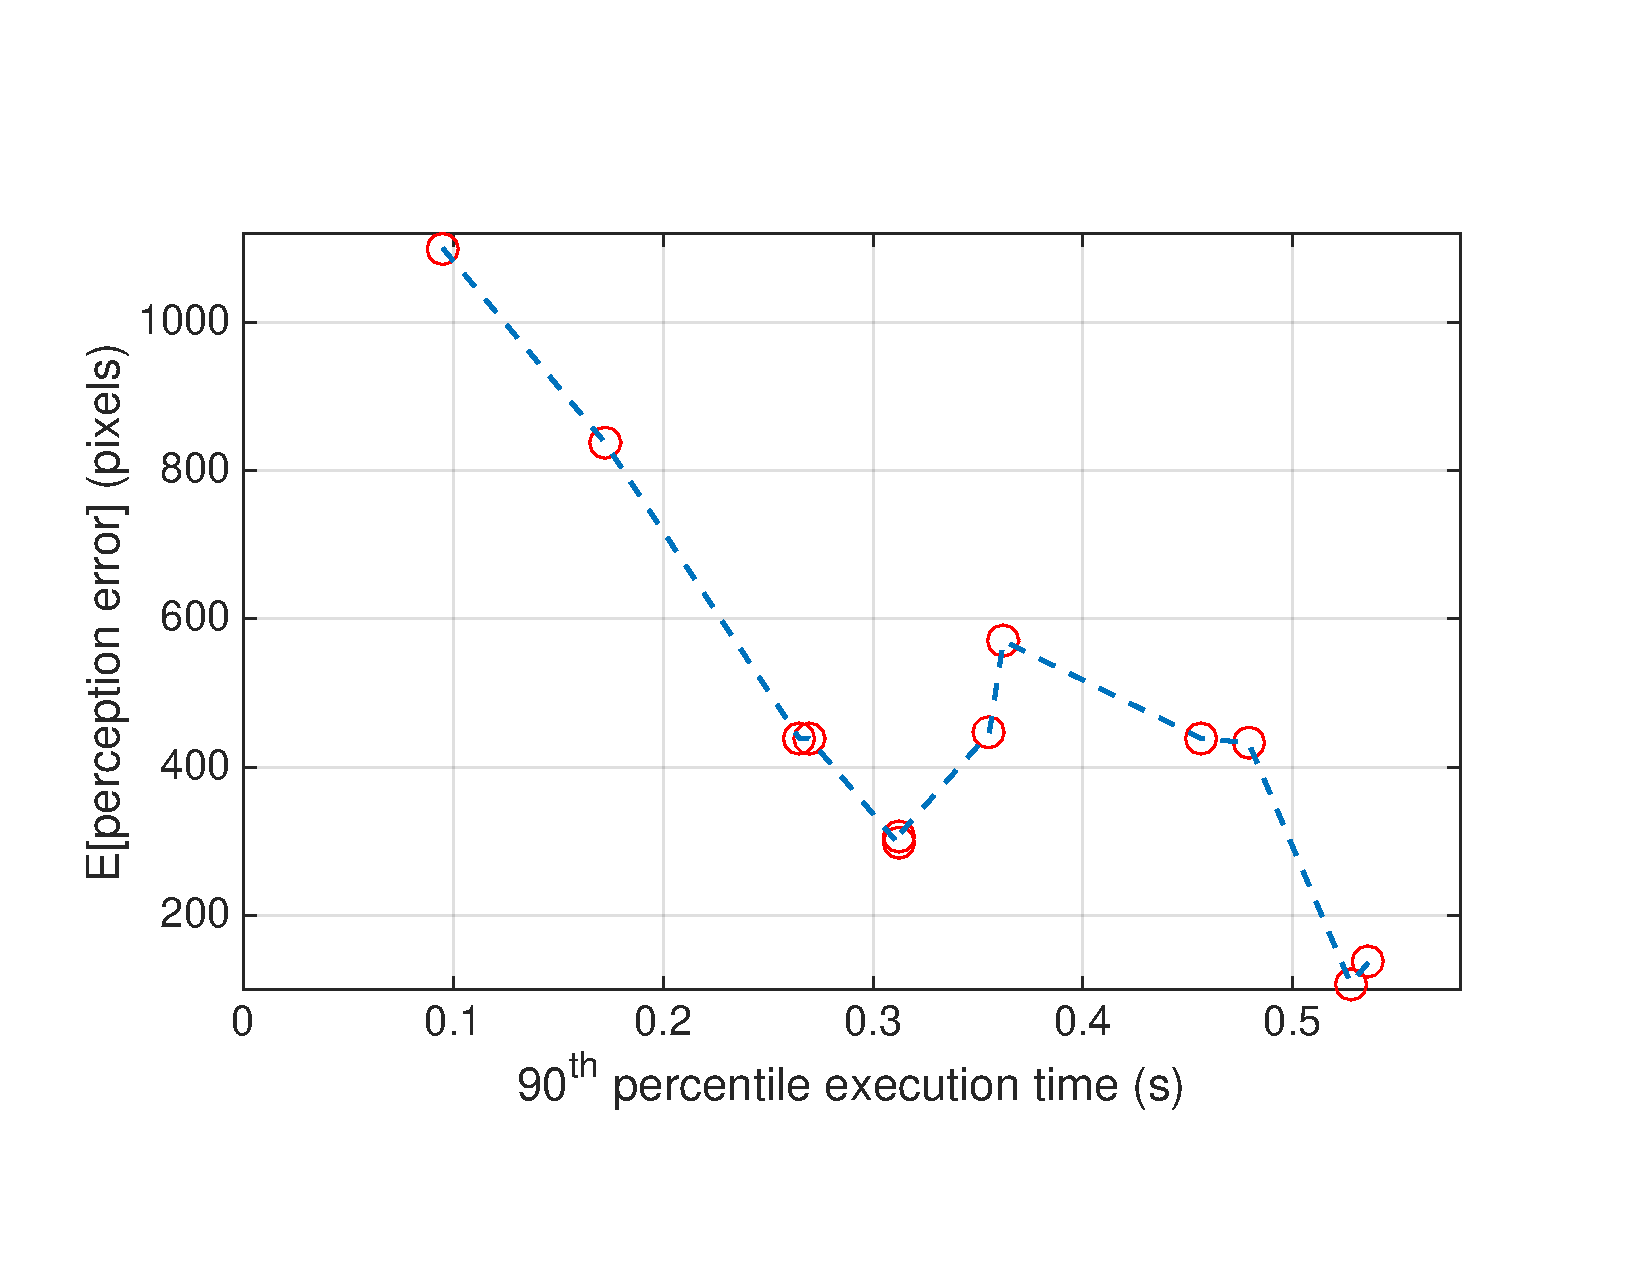
\includegraphics[width=0.7\linewidth]{figures/chainErrorDelay}
	\caption{Perception error vs Delay curve for the chain of Fig.~\ref{fig:chain}}
	\label{fig:chainErrorDelay}
\end{figure}
More generally, such curves can be obtained for a given state estimator by identifying the knobs that control the quality and runtime of the estimator, and profiling the estimator's code at the various values of the knobs.
In effect, this gives us several Estimator tasks, each with a different utility. 
I.e., each such task strikes a different balance between computation time and quality of estimate.
At time step $k$, the controller schedules the task with the best trade-off for step $k+1$, in the sense of optimizing the cost function in Eq.??



	\section{Case Study: Real-time feedback control of a hex-rotor with contract based estimation and robust control}
\label{experiments}

To evaluate our methodology on a real platform, we applied it to a hex-rotor tasked with following a given trajecotory. The hex-rotor flies using visual odometry from a downward facting camera for self-localization and using our Robust Model Predictive Algorithm for both the position control of the hex-rotor and setting the time deadline for the visual odometry computations. For the contract based perception and estimation algorithm we use the FAST corner detector (as in section \ref{}) providing measurements to an Unscented Kalman Filter that also uses measurements from an Inertial Measurement Unit (IMU) to provide a state estimate for the control algorithm to use.
In the following section we show how our approach dynamically schedules different modes of the contract-based perception and estimation algorithm at run-time and also controls the dynamic system in an energy efficient order while providing good tracking performance. In the evaluation subsection we will compare our results to a baseline Model Predictive Control algorithm that does not leverage co-design and operates at fixed ($\delta,\epsilon$) points of the perception/estimation algorithm which provides a state estimate to the controller. 

\subsection{Experimental setup}
\todo[inline]{details about hex-rotor and odroid and the visual odometry. Figure for control/percpetion architecture of hex-rotor here, cvxgen based rampc}
%Hexrotor \textbf{<specs here>} using visual odometry from a downward facing camera. Figure for hexrotor, figure for images from hexrotor downward facing, and figure for hexrotor control architecture.  
\todo[inline]{Plant model and estimation here}
%We illustrate the foregoing results on the hexarotor example from Section \ref{motivatingExample}.
%Recall that we found the control performance, as measured by $J$ of Eq.??, to degrade as the robot's speed was increased.
%We implemented the RAMPC controller of Section \ref{controlProblem}, and used the error-delay curves of Section \ref{delayErrorCurve}.


\subsection{Profiling the perception and algorithm toolchain}

Recall that in section \ref{}, the control algorithm needs the profiled ($\delta,\epsilon$) curve for the perception and estimation algorithm. In this setup, as described in figure \ref{}, we need to the performance of the FAST detector based visual odometry. Figure \ref{} shows the bound on estimation error and the $90^{th}$ percentile execution times for a different number of maximum corners in the FAST detector through extensive flying over a relatively feature rich environment (figure \ref{}). The estimation error is computed with the help of ground truth obtained through the VICON system. We can profile the performance for the same flights with different settings of the odometry offline by logging images and IMU data in-flight, and then running the visual odometry code on the odroid offline and playing back the camera and IMU data in the form of a ROSBAG (\ref{}) from a separate machine running ROS. \todo[inline]{more details here, Kartik?}
This accurately recreates the in flight environment that is present for the FAST corner detector based visual odometry and this profiling done offline is then used online for making in flight decisionsby the control algorithm.

Also needed for the control optimization as stated in equation \ref{} is a measure of the power consumption by the visual odometry while at different settings on maximum number of corner. This is obtained again by running the visual odomery code offline for different knob settings and measuring the power consumed by the Odroid to perform these computations. Power measurements are made using the Odroid Smart Power meter \cite{OdroidSmartPower}, which measures consumption at 10Hz to milliwatt precision. We measure the power consumption of the entire Odroid board, including CPU and DRAM power consumption. To avoid the physical challenges of fitting the power meter onto our hex-copter platform, we measure the power consumption of the Odroid board on the ground, running the same controller and vision workloads as it does during flight as explained above.

This offline profiling now allows us to formulate the co-design problem for the hex-rotor and experimentally evaluate our methods.




\begin{figure}[htbp]
  \centering
  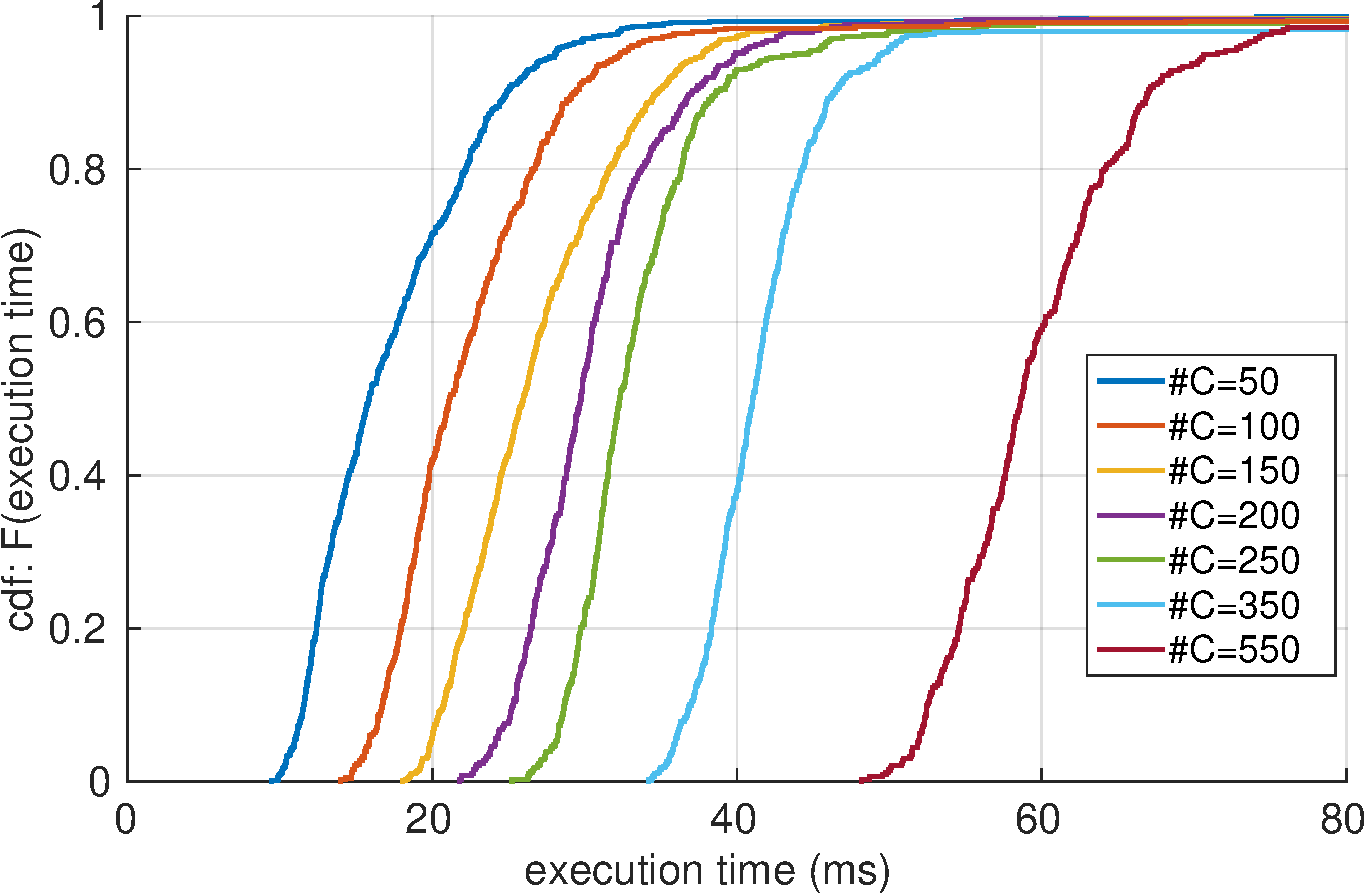
\includegraphics[width=0.45\textwidth]{figures/time_ecdf_millisec.pdf}
  \caption{Cumulative distribution of profiled execution times for visual odometry running on the Odroid U-3 for varying maximum number of corners from the FAST detector.}
\end{figure}

Fig.~\ref{fig:modeSwitching} shows that the RAMPC indeed chooses different modes, indicating that awareness of the error/delay trade-off does lead to improved performance.
\begin{figure}[t]
	\centering
	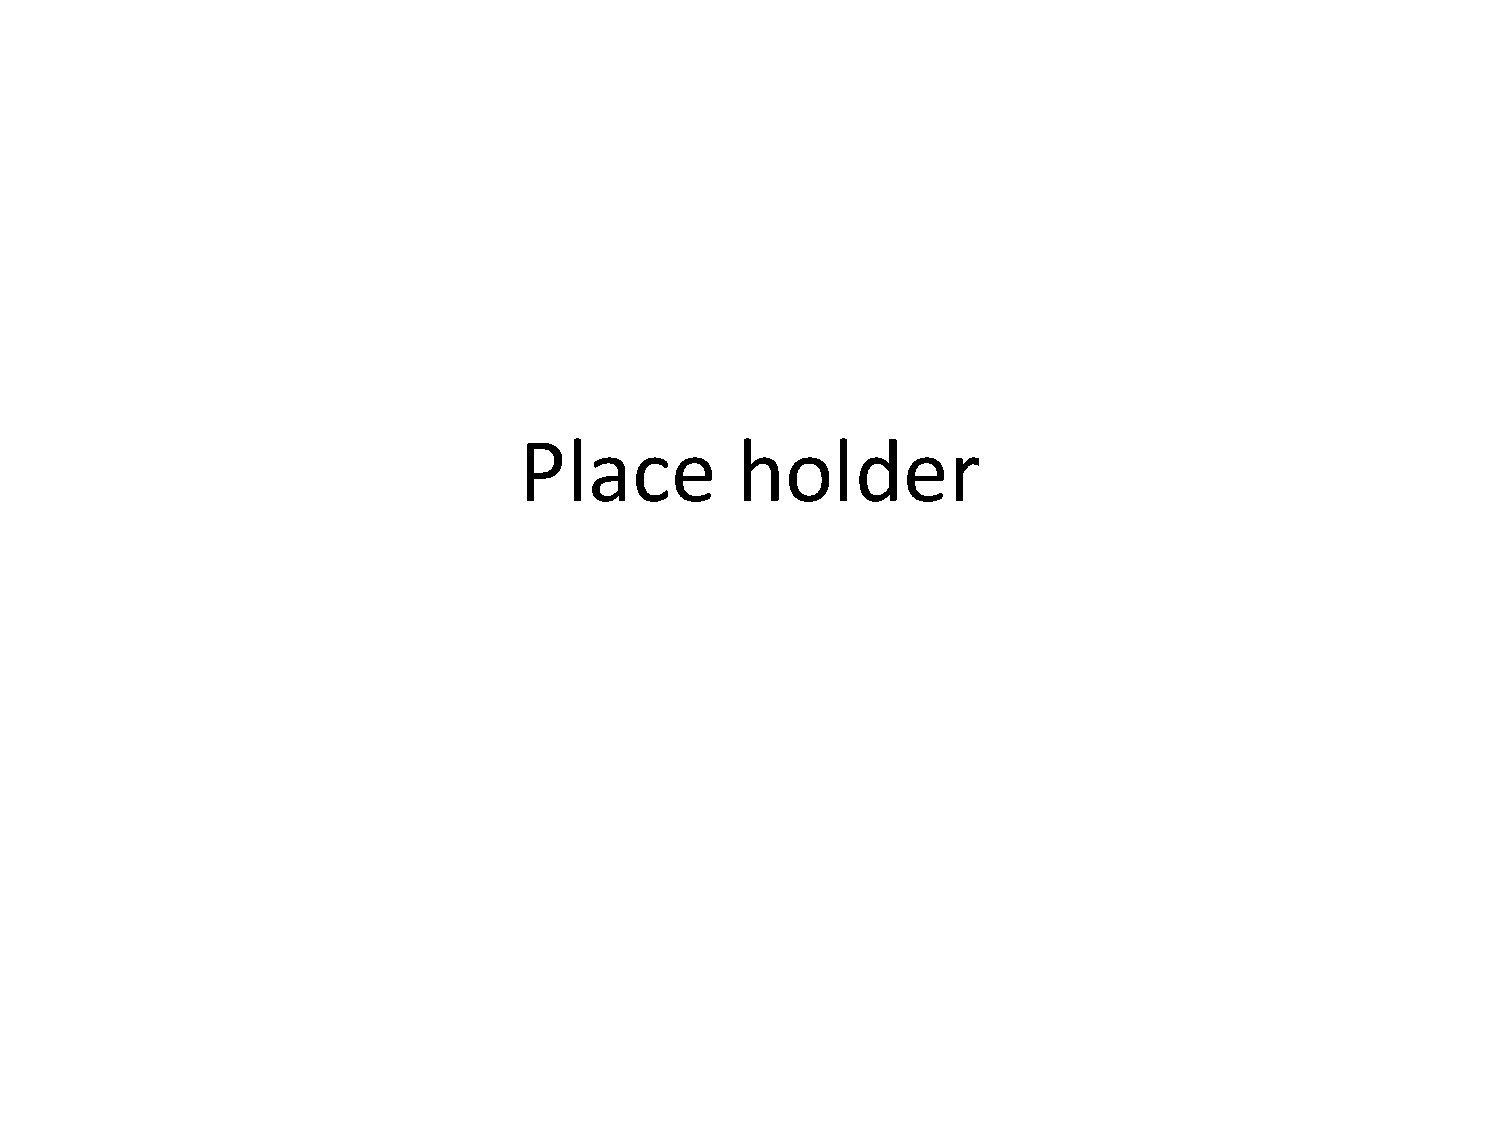
\includegraphics[width=0.7\linewidth]{figures/placeHolder}
	\caption{Mode switches of RAMPC.}
	\label{fig:modeSwitching}
\end{figure}


\subsection{Experimental Evaluation}

After profiling the performance of the perception and estimation algorithm and formulating the Robust MPC controller for the hex-rotor model (equation \ref{}), we experimentally evaluate the tracking performance and estimated energy consumption based on actual flights around a pre-defind trajectory. For comparision, we use a Model Predictive Controller with the same cost function and initial feasible sets as in our Robust MPC formulation. Comparision to such a controller would give a baseline to measure the benefits of our co-design method against the a similar control algorithm that does not leverage co-design and is unaware of the estimator algorithm that gives it a state estimate. 

For the evaluation, we fly in a predefined trajectory as shown in figure \ref{}, repeating the experiment 10 times to gather enough data to conclusively measure the performance of Robust MPC and MPC with fixed modes of ($\delta,\epsilon$). Note that since the controller was a sampled discrete-time controller working with simulated 20Hz camera updates, this realistically restricts us to using modes of estimator operation with delay ($\delta$) less than (1/20s), or one sampling period, i.e. modes corresponding to 50, 100, 150 and 200 maximum corners from the FAST detector (see figure \ref{fig:svo_error_delay}). These modes and their estimated power consumption is in table \ref{tbl:modes_exp}. Note, \#C represents maximum number of FAST corners requested, $\epsilon$ shows the worst case error bound on the state estimate, $\delta$ is the $90^{th}$ percentile execution time for that mode, and $P$ represents the expected power consumption in that mode as profiled offline. This power consumption is the computation power used by a particular mode in excess to the idle power for the Odroid used for profiling, which was 1.5W.

\begin{table}[htb]
\begin{center}
\caption{Estimation modes used in the experiment.}
\label{tbl:modes_exp}
\begin{tabular} {|c|c|c|c|c|}
	\hline
	\textbf{Mode} & \textbf{\#C} & $\pmb{\epsilon}$ & $\pmb{\delta}$ \textbf{(ms)} & $\pmb{P}$\textbf{(W)} \\ \hline
	0 & 50 &  24.88 & 0.028 &  0.778  \\ \hline
 	1 & 100 & 29.82 & 0.0237 &  0.862  \\ \hline
	2 & 150 & 34.66 & 0.0230 & 0.870 \\ \hline
	3 & 200 & 38.01 & 0.0113 & 0.951 \\ \hline
	\end{tabular}	
	\end{center}
\end{table}




\subsection{Experimental Results}

Once the flights are complete, to get a more accurate picture of how the controllers really performed, we use the following function to measure tracking performance at each time step.

\begin{equation}
	J_{true}(t) =  (x(t)-x_{ref}(t))^{T}Q(x(t)-x_{ref}(t)) + u(t)^{T}Ru(t)
\end{equation}

Note that since we have access to the true position and velocities ($x(t)$) of the hexrotor with the VICON system, we can obtain the true tracking cost. Table \ref{tbl:RAMPC_MPC_performance} shows the mean of the above function over the 10 flights for both MPC across all fixed modes and RAMPC with different values of $\alpha$. It also shows the estimated energy consumption based on the time spent in each mode (which can be seen in Table \ref{tbl:RAMPC_ModeTime} for RAMPC). RAMPC shows better tracking performance (lower mean $J_{true}$) than the MPC with either of the 4 fixed modes, showing the improved control performance that can be obtained by dynamically switching between estimation modes in-flight at runtime. 

\begin{figure}[tbh]
	\centering
	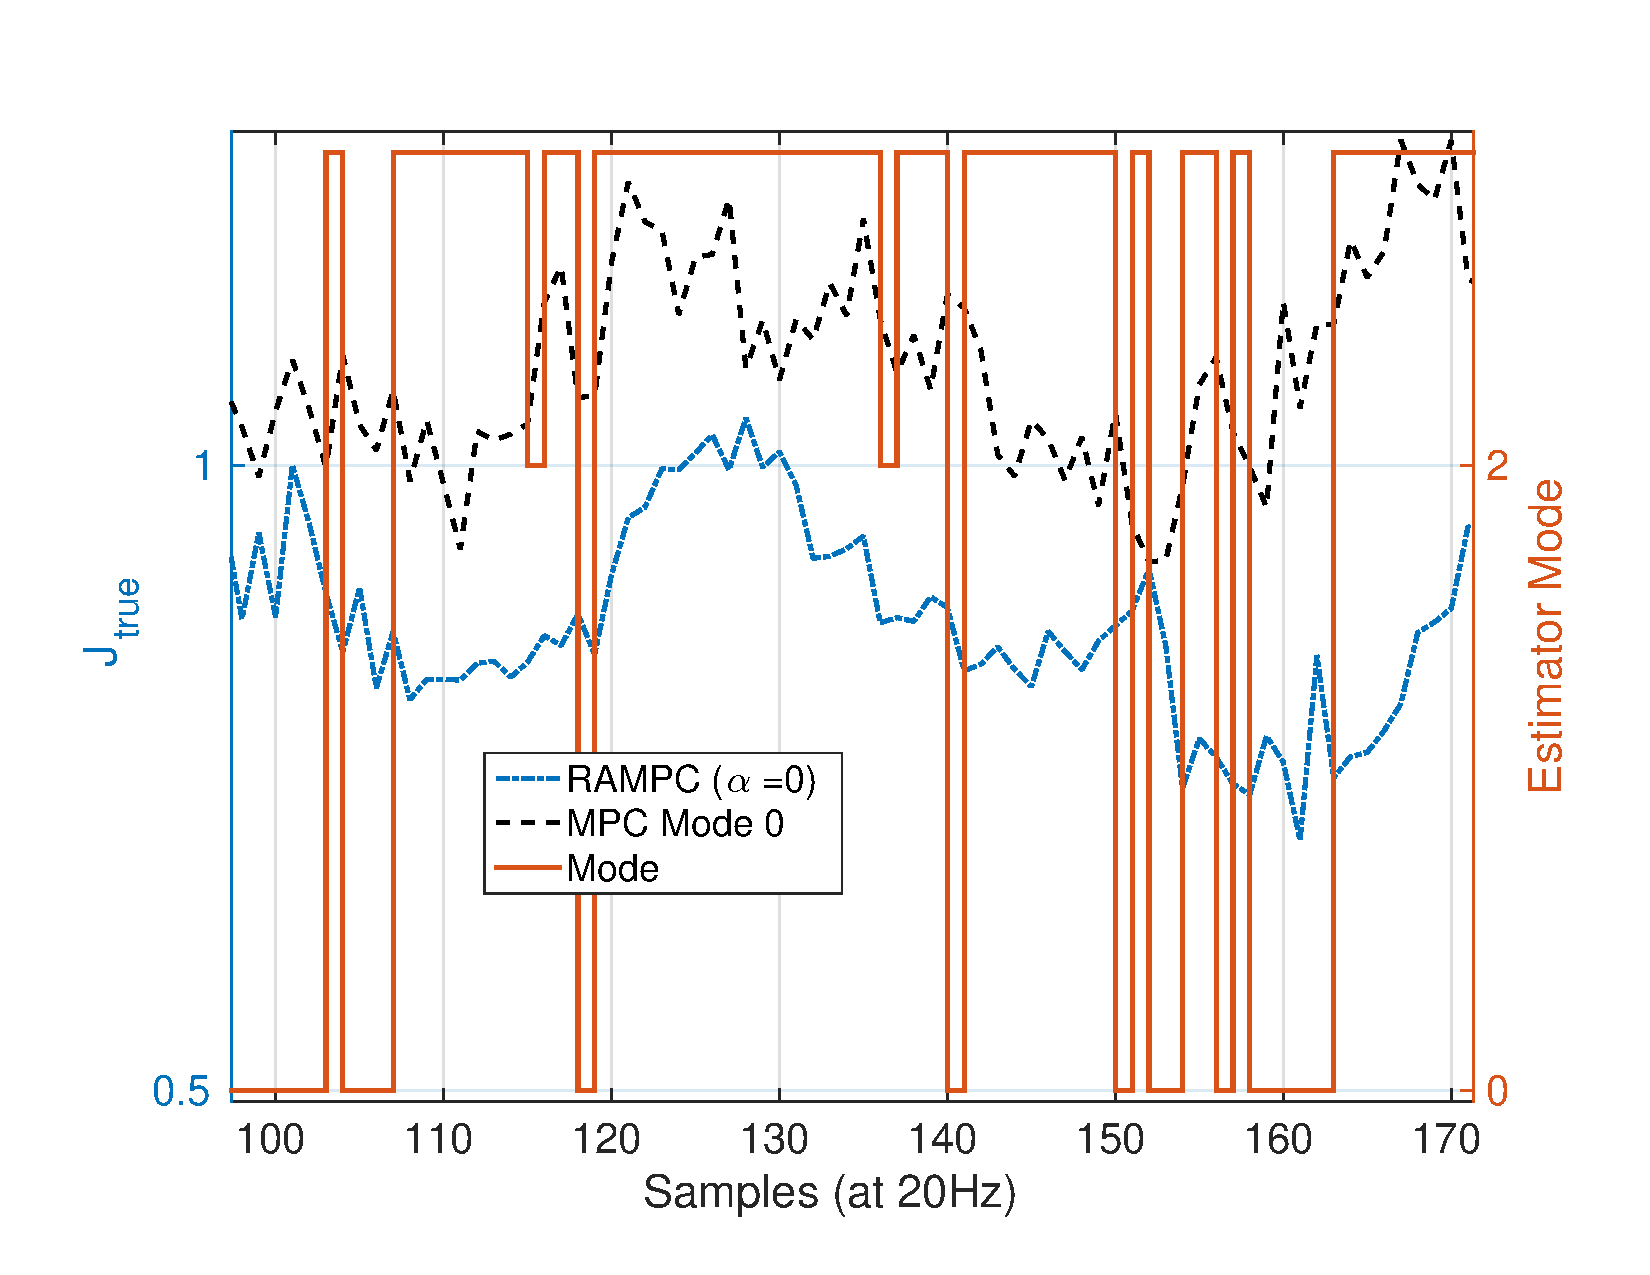
\includegraphics[width=0.49\textwidth]{figures/CostAndModes}
	\caption{Tracking cost at each time step for MPC (fixed mode 0 estimator) and RAMPC with $\alpha=0$. Note how the RAMPC performs better (lower cost) than the MPC and there is dynamic switching of estimator modes at runtime leading to improved performance for the RAMPC.}	
	\label{fig:CostAndModes}
\end{figure}


Figure \ref{fig:CostAndModes} shows how the tracking cost ($J_{true}$) evolves over time for RAMPC (with $\alpha=0$) and MPC (fixed mode 0) for a portion of the hexrotor flight. The estimator modes selected by RAMPC are overlaid in orange. Figure \ref{fig:CostAndModes} demonstrates that RAMPC has uniformly lower tracking cost than MPC, enabled by RAMPC's dynamic switching of estimator modes at runtime. Note that RAMPC exhibits better tracking performance throughout the flight and not just in this portion, and also outperforms MPC at other modes (see Table \ref{tbl:RAMPC_MPC_performance}).

Figure \ref{fig:TrackingVsEnergy} shows that RAMPC provides better tracking performance while using less energy to do so. For any fixed energy budget (a point on the x-axis), RAMPC delivers lower tracking cost (y-axis) than MPC. While MPC's tracking error is relatively constant across modes, RAMPC is able to balance tracking error with energy consumption by varying the $\alpha$ parameter. RAMPC's switching between estimation modes improves not only the control performance but also energy efficiency.


\begin{figure}[tbh]
	\centering
	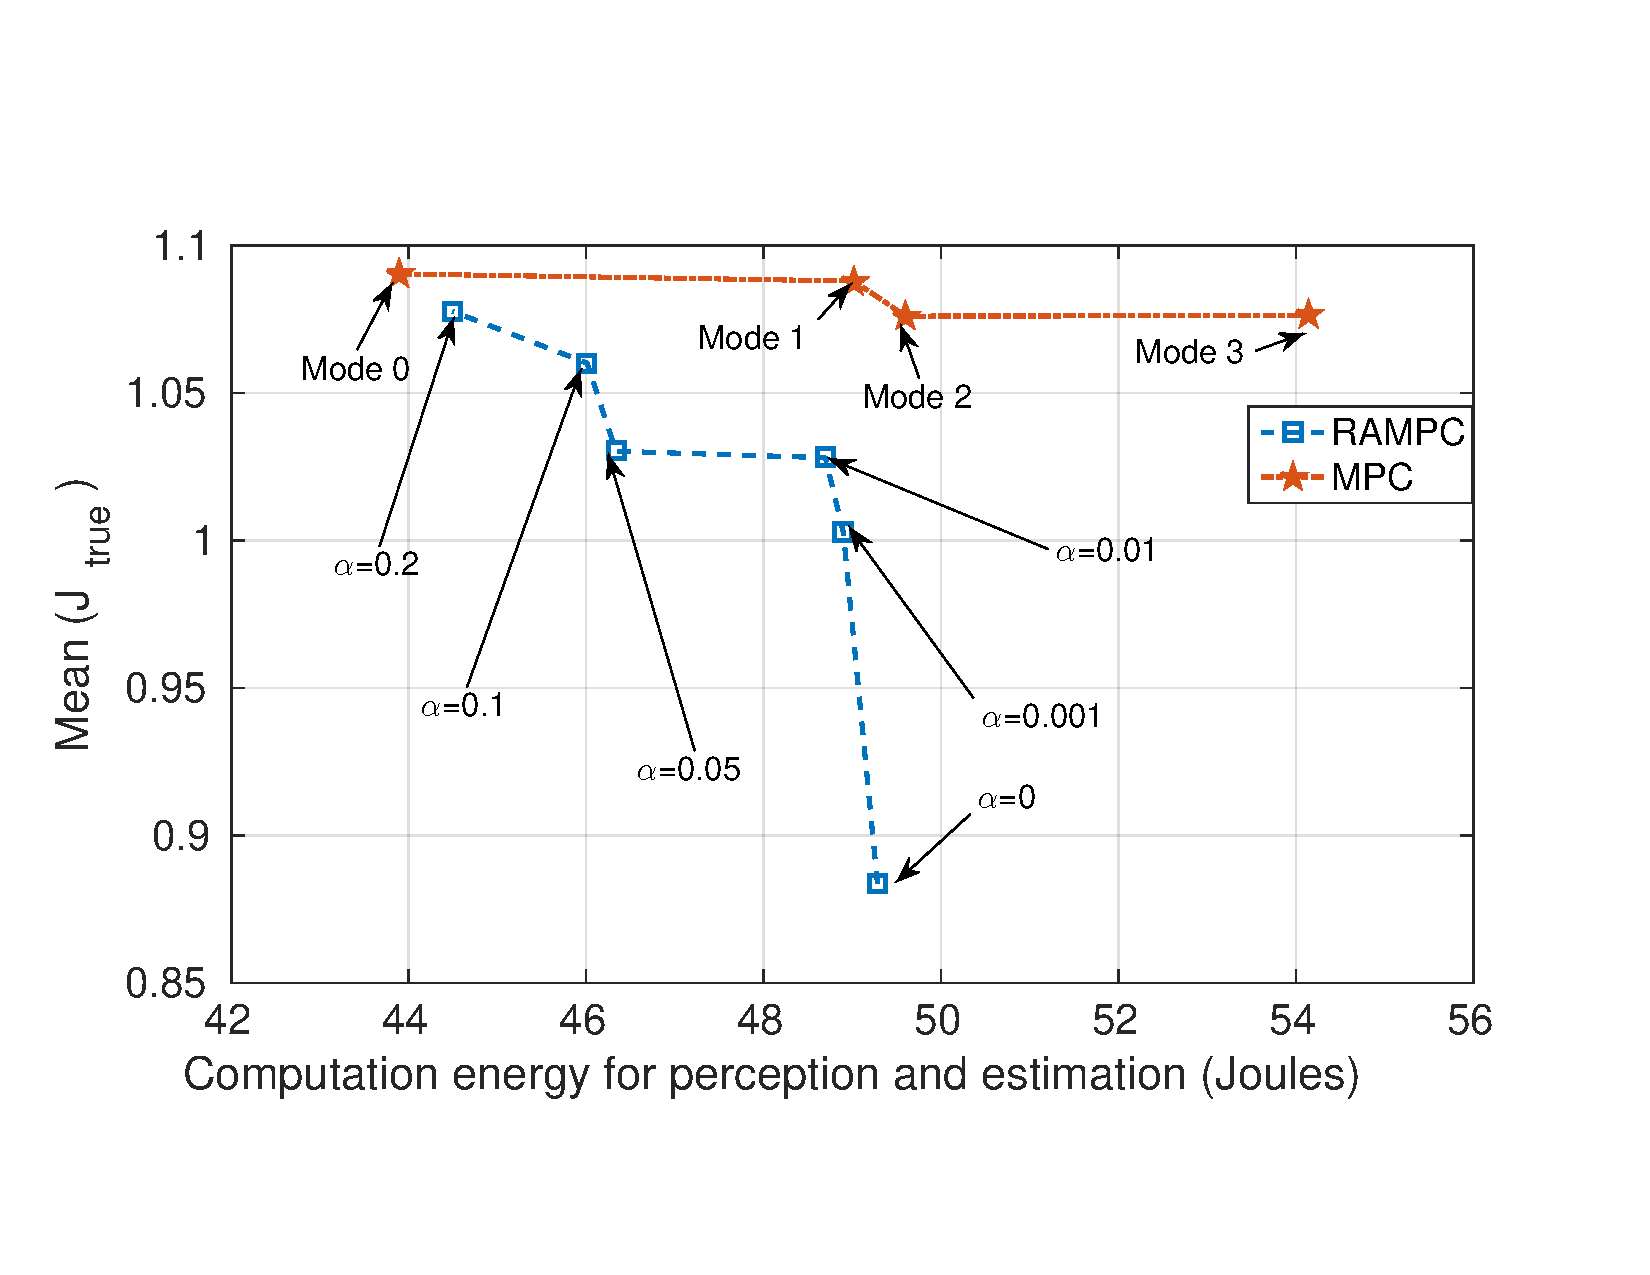
\includegraphics[width=0.49\textwidth]{figures/TrackingVsEnergy}
	\caption{Tracking cost vs estimated computation energy for executing the perception and estimation algorithm. Note for MPC, different energies are realized only by operating at different fixed modes of the perception and estimation algorithm. Using RAMPC as the controller, the different energies are due to run-time scheduling of different modes based on the optimal value of the cost function of Eq. \ref{eq:tractableOptim} at each time step based on different values of $\alpha$. It is worth noting that RAMPC with co-design outperforms standard MPC on tracking performance across the entire range of energy consumption.}
	\label{fig:TrackingVsEnergy}
\end{figure}


\begin{table}[htb]
\begin{center}
\caption{Tracking performance and computation energy}
\label{tbl:RAMPC_MPC_performance}
\begin{tabular} {|c|c|c|c|c|}
	\hline
	\textbf{Controller} &\textbf{Est. Mode}/ $\pmb{\alpha}$ & $\pmb{E[J_{true}]}$ & $\pmb{\sigma({J_{true}})}$ & $\pmb{Energy(J)}$ \\ \hline
	MPC & 0/ $-$ & 1.0903 & 0.104 & 43.89\\ \hline
	MPC & 1/ $-$ & 1.0878 & 0.087 & 49.02 \\ \hline
	MPC & 2/ $-$ & 1.0760 & 0.098 & 49.60 \\ \hline
	MPC & 3/ $-$ & 1.0762 & 0.088 & 54.15 \\ \hline
	RAMPC &  $-$/0 & 0.8836 & 0.079 & 49.28 \\ \hline
	RAMPC & $-$/ 0.001 & 1.0029 & 0.093 & 48.90  \\ \hline
	RAMPC & $-$/ 0.01 & 1.0280 & 0.089 & 48.69  \\ \hline
	RAMPC & $-$/ 0.05 &1.0302 & 0.096 & 46.33 \\ \hline
	RAMPC & $-$/ 0.1 &1.0601 & 0.086 & 46.01 \\ \hline
	RAMPC & $-$/ 0.2 & 1.0776 & 0.083 & 44.49 \\ \hline
\end{tabular}	
	\end{center}
\end{table}



Figure \ref{fig:CostAndEnergyVsAlpha} shows the degradation (increased mean $J_{true}$) in tracking performance and reduction in energy consumption as the weight $\alpha$ for the computation power consumption in the cost function is increased. As energy becomes more important, RAMPC smoothly balances tracking cost and energy consumption. Table \ref{tbl:RAMPC_ModeTime} quantifies how RAMPC makes this trade-off, by showing the fraction of time spent in the 4 modes with RAMPC as $\alpha$ changes. While time is split between modes 0 and 3 with $\alpha=0$, more and more time is spent in the low-power (but less accurate) mode 0 as $\alpha$ increases.


\begin{figure}[t]
	\centering
	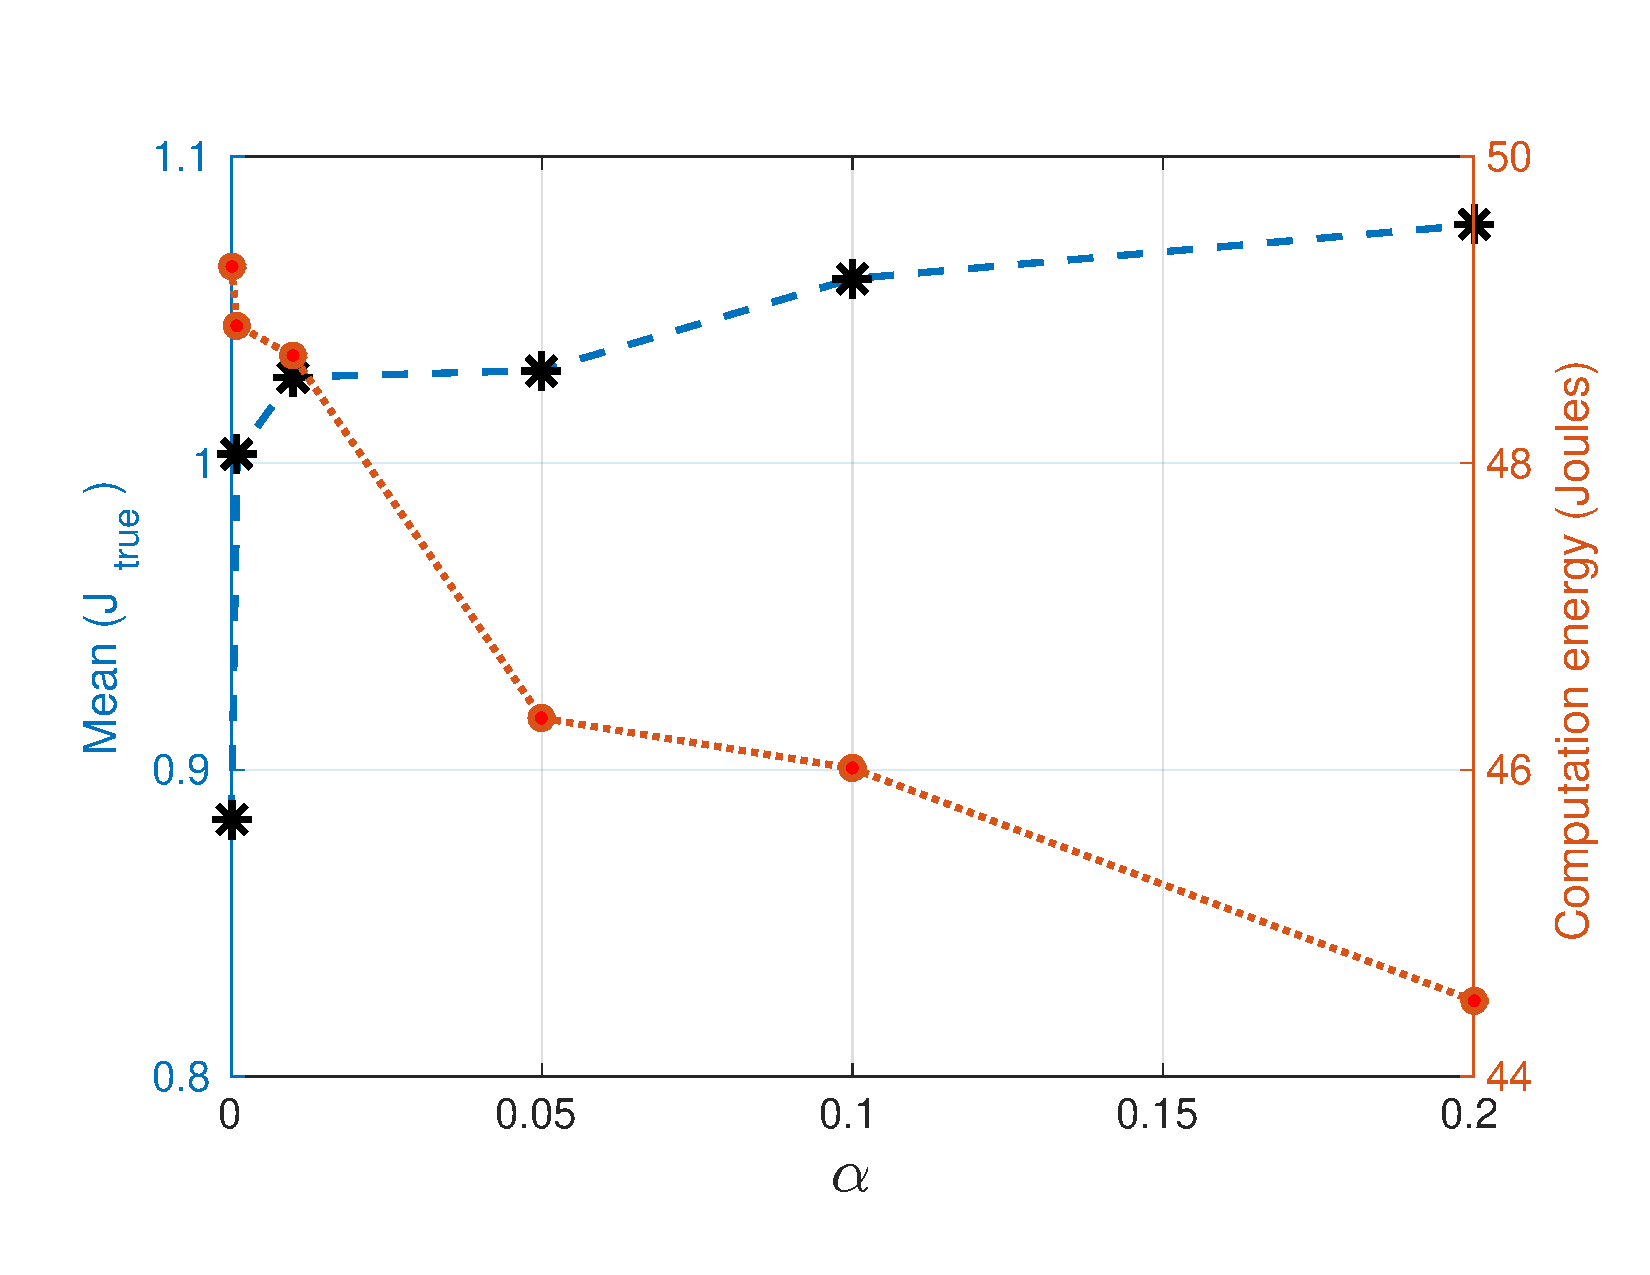
\includegraphics[width=0.49\textwidth,scale=0.7]{figures/CostAndEnergyVsAlpha}
        \vspace{-20pt}
	\caption{RAMPC tracking cost and estimated computation energy for the perception and estimation algorithm as a function of $\alpha$. }
	\label{fig:CostAndEnergyVsAlpha}
\end{figure}


\begin{table}[htb]
\begin{center}
\caption{Fraction of time spent in different estimator modes as $\alpha$ changes for RAMPC}
\label{tbl:RAMPC_ModeTime}
\begin{tabular} {|c|c|c|c|c|}
	\hline
	$\pmb{\alpha}$ & \textbf{Mode 0} & \textbf{Mode 1} & \textbf{Mode 2} & \textbf{Mode 3} \\ \hline
	0 & 0.461 & 0.009 & 0.020 & 0.510 \\ \hline
 	0.001 &  0.494 & 0.001 & 0.029 & 0.467 \\ \hline
	0.01 & 0.512 & 0.005 & 0.039 & 0.444  \\ \hline
	0.005 &  0.692 & 0.000 & 0.156 & 0.152 \\ \hline
	0.1 & 0.691 & 0.000 & 0.218 & 0.091 \\ \hline
	0.2 & 0.897 & 0.000 & 0.098 & 0.005  \\ \hline
	\end{tabular}	
	\end{center}
\end{table}



	\section{Conclusion}
\label{conclusion}

In this paper we presented a contract-based methodology for co-design of estimation and control for autonomous systems. 
The basic idea is that the control algorithm requests a time and estimation error $\de$ contract that the perception-and-estimation algorithm realizes. The control algorithm we designed aims to set time varying contracts to maximise a performance function while guaranteeing feasibility constraints and stability under the time varying execution time and estimation error from the estimator. We also illustrate how the contract based perception-and-estimation algorithm is designed offline and used at run-time to best meet the $\de$ contracts set for it. Through a case study on a flying hex-rotor, we showed the applicability of our scheme to real-time closed loop system. The experimental results show the good performance of our scheme and how it outperforms regular Model Predictive Control which does not leverage co-design. A key result showed how our closed loop solution is more energy efficient than MPC while achieving better tracking performance. A focus of ongoing research is to overcome the necessity of the contracts always being met by the estimator in order of us to have strong mathematical guarantees for the control performance. Another focus is on an automated tool chain to profile perception algorithms commonly used in autonomous systems.
	
	\section*{Acknowledgements}
	We would like to thank Kuk Jang for his help in creating several of the diagrams in this paper.
	\bibliographystyle{IEEEtran}%abbrv}
	\bibliography{IEEEabrv,rtss2015,cdc14,anytime_ref}

	%\section*{Appendix}
\label{appendix}

In this appendix we give the detailed mathematical derivation of the results of Section \ctrlProbSecRef.
The controller is designed using a Robust Model Predictive
Control (RMPC) approach via constraint restriction \cite{richardsetal05rmp, chiscietal01swp}, 
and augments it by an adaptation to the error-delay curve of the estimator.
In order to ensure robust safety and feasibility, the key idea of
the RMPC approach is to tighten the constraint sets iteratively to account
for possible effect of the disturbances. 
As time progresses, this ``robustness
margin'' is used in the MPC optimization with the nominal dynamics,
i.e., the original dynamics where the disturbances are either removed
or replaced by nominal disturbances.
%An advantage of this approach is that, 
Because only the nominal dynamics are used, the complexity of the optimization is the same as for the nominal problem.

Since the controller only has access to the estimated state $\hat{x}$, we need
to rewrite the plant's dynamics with respect to $\hat{x}$. 
The error
between $ $$x_{k}$ and $\hat{x}_{k}$ is $e_{k}=x_{k}-\hat{x}_{k}$.
At time step $k+1$ we have
\begin{align*}
\hat{x}_{k+1} & =x_{k+1}-e_{k+1}\\
 & =Ax_{k}+B_{1}(\sDelay_k)u_{k-1}+B_{2}(\sDelay[k])u_{k}+w_{k}-e_{k+1}\text{,}
\end{align*}
 then, by writing $x_{k}=\hat{x}_{k}+e_{k}$, we obtain the dynamics
\begin{equation}
\hat{x}_{k+1}=A\hat{x}_{k}+B_{1}(\sDelay[k])u_{k-1}+B_{2}(\sDelay[k])u_{k}+\hat{w}_{k}\label{eq:estimator-dynamics}
\end{equation}
 where $\hat{w}_{k}=w_{k}+Ae_{k}-e_{k+1}$.
The set of possible values of $\hat{w}_{k}$
depends on the estimation accuracy at steps $k$ and $k+1$ and is
denoted by $\hWc(\sAccu[k],\sAccu[k+1])$, i.e.,
$\hWc(\sAccu,\sAccu')\defeq \left\{ w+Ae-e'\sut w\in\Wc,e\in\ESet(\sAccu),e'\in\ESet(\sAccu')\right\}$.
Note that %we assume
$\hWc(\sAccu[k],\sAccu[k+1])$ is independent
of the time step $k$. %
It can be computed as $\hWc(\sAccu,\sAccu')=\Wc\oplus A\ESet(\sAccu)\oplus\left(-\ESet(\sAccu')\right)$
where the symbol $\oplus$ denotes the Minkowski sum of two sets.

The dynamics in \eqref{eq:estimator-dynamics} has a non-standard form
where it depends on both the current and the previous control inputs.
However we can expand the state variable to store the previous control
input as
\[
\hat{z}_{k}=\begin{bmatrix}\hat{x}_{k}\\
u_{k-1}
\end{bmatrix}\in\Re^{n+m}
\]
and rewrite the dynamics as, for all $k\geq0$,
\begin{equation}
\hat{z}_{k+1}=\hat{A}(\sDelay_k)\hat{z}_{k}+\hat{B}(\sDelay_k)u_{k}+\hat{F}\hat{w}_{k}\text{.}\label{eq:estimator-std-dynamics}
\end{equation}
Here, the system matrices are
\begin{equation}
\begin{gathered}
\hat{A}(\sDelay_k)=\begin{bmatrix}A & B_{1}(\sDelay_k)\\
\bm{0}_{m\times n} & \bm{0}_{m\times m}
\end{bmatrix},\\
\hat{B}(\sDelay_k)=\begin{bmatrix}B_{2}(\sDelay_k)\\
\IdentityMatrix_{m}
\end{bmatrix},\quad\hat{F}=\begin{bmatrix}\IdentityMatrix_{n}\\
\bm{0}_{m\times n}
\end{bmatrix}\text{.}
\end{gathered}
\label{eq:lifted-matrices}
\end{equation}

Let the actual expanded state be $z_{k}=\left[x_{k}^{T},u_{k-1}^{T}\right]^{T}$.
Because the expanded state consists of both the plant's state and
the previous control input, the state constraint $x_{k}\in\stSet$
and the control constraint $u_{k}\in\inpSet$ are equivalent to the
joint constraint $z_{k}\in\stSet\times\inpSet$. We can now describe
the RAMPC algorithm for the dynamics in \eqref{eq:estimator-std-dynamics}.

\subsection{Tractable RAMPC Algorithm}

Let $N\geq1$ be the horizon length of the RMPC optimization. 
Because the system
matrices in the state equation~(\ref{eq:estimator-std-dynamics})
depend nonlinearly on the variables $\sDelay_k$, the RMPC optimization
is generally a mixed-integer nonlinear program, which is very hard
to solve. To simplify the RMPC optimization to make it tractable, we fix the estimation mode for the entire RMPC horizon.

Let $\RAMPCProb{\de}{k}$
denote the RMPC optimization problem at step $k\geq0$ where the current
state estimate is $\hat{x}_{k}$, the current estimation mode is $(\sDelay_k,\sAccu_k)\in\Delta$,
the previous control input is $u_{k-1}$, and the estimation mode
for the entire horizon (after step $k$) is fixed at $(\sDelay,\sAccu)\in\Delta$.
Since the system matrices become constant now, if the stage cost $\ell(\cdot)$
is linear or positive semidefinite quadratic, each optimization problem
$\RAMPCProb{\de}{\cdot}$ is tractable and can be solved
efficiently as we will show later. 
The RAMPC algorithm with Anytime Estimation is stated in Alg. \algoref.

\subsection{RMPC Formulation}

We formulate the RMPC optimization $\RAMPCProb{\de}{k}$
with respect to the nominal dynamics, which is the original dynamics
in \eqref{estimator-std-dynamics} but the disturbances are either
removed or replaced by nominal disturbances. 
To ensure robust feasibility
and safety, the state constraint set is tightened after each step
using a candidate stabilizing state feedback control, and a terminal
constraint is derived. 
In this RMPC formulation, we extend the approach
in \cite{richardsetal05rmp, chiscietal01swp}. 
At time step $k$, given
$(\hat{x}_{k},\sDelay_k,\sAccu_k,u_{k-1})$ and for a fixed $(\sDelay,\sAccu)$,
we solve the following optimization 

\begin{subequations}
	\label{eq:RMPC1}
 \begin{equation} J_{\sDelay,\sAccu}^{*} \left(\hat{x}_{k},\sDelay_k,\sAccu_k,u_{k-1}\right) = \min_{\boldsymbol{u},\boldsymbol{x}}\sum_{j=0}^{N}\ell(\Nom x_{k+j\Given k},u_{k+j\Given k})
 \end{equation}
 \begin{equation}
  \text{subject to, }\forall j\in\left\{ 0,\dots,N\right\} \nonumber 
 \end{equation}
 \begin{equation}
  \Nom z_{k+j+1\Given k}=\hat{A}(\sDelay_{k+j\Given k})\Nom z_{k+j\Given k}+\hat{B}(\sDelay_{k+j\Given k})u_{k+j\Given k}\label{eq:RMPC1-dyn}
 \end{equation}
 \begin{equation}
  ( \sDelay_{k+j+1\Given k},\sAccu_{k+j+1\Given k} ) \!=\! (\sDelay,\sAccu ) \nonumber
 \end{equation}
 \begin{equation}
  (\sDelay_{k\Given k},\sAccu_{k\Given k}) \!=\! (\sDelay_k,\sAccu_k)  \label{eq:RMPC1-delay}
 \end{equation}
 \begin{equation}
  \Nom x_{k+j\Given k}=\begin{bmatrix}\IdentityMatrix_{n} \quad \bm{0}_{n\times m}\end{bmatrix}\Nom z_{k+j\Given k}\label{eq:RMPC1-z2x}
 \end{equation}
 \begin{equation}
  \Nom z_{k\Given k}=\left[\hat{x}_{k}^{T},u_{k-1}^{T}\right]^{T} \label{eq:RMPC1-z0}
 \end{equation}
 \begin{equation}
  \Nom z_{k+j\Given k}\in\ZSet_{j}\left(\sAccu_k,\sAccu\right)\label{eq:RMPC1-zset}
 \end{equation}
 \begin{equation}
  \Nom z_{k+N+1\Given k}\in\ZSet_{f}\left(\sAccu_k,\sAccu\right) \label{eq:RMPC1-zfinalset}
  \end{equation}
\end{subequations} 

in which $\Nom z$ and $\Nom x$
are the variables of the nominal dynamics. The constraints of the
optimization are explained below.
\begin{itemize}
\item \eqref{eq:RMPC1-dyn} is the nominal dynamics.
\item \eqref{eq:RMPC1-delay} states that the estimation mode is fixed at $\left(\sDelay,\sAccu\right)$
except for the first time step when it is $\left(\sDelay_k,\sAccu_k\right)$.
\item \eqref{eq:RMPC1-z2x} extracts the nominal state $\Nom x$ of the plant
from the nominal expanded state $\Nom z$.
\item \eqref{eq:RMPC1-z0} initializes the nominal expanded state at time step
$k$ by stacking the current state estimate and the previous control
input.
\item \eqref{eq:RMPC1-zset} tightens the admissible set of the nominal expanded
states by a sequence of shrinking sets.
\item \eqref{eq:RMPC1-zfinalset} constrains the terminal expanded state to
the terminal constraint set $\ZSet_{f}$.
\end{itemize}

\noindent\textit{The state constraint $\ZSet_{j}$:}
%
The tightened state constraint sets $\ZSet_{j}\left(\sAccu_k,\sAccu\right)$
are parameterized with two parameters $\sAccu_k$ and $\sAccu$.
They are defined as follows, for all $j\in\left\{ 0,\dots,N\right\} $
\begin{eqnarray}
\ZSet_{0}(\sAccu_k,\sAccu)=\ZSet\ominus\hat{F} \ESet(\sAccu_k)\label{eq:RMPC1-Z0}
\\
\ZSet_{j+1}(\sAccu_k,\sAccu)=\ZSet_{j}(\sAccu,\sAccu)\ominus L_{j}\hat{F}\hWc(\sAccu_k,\sAccu)\label{eq:RMPC1-Zj}
\label{eq:RMPC1-Z}
\end{eqnarray} 
in which the symbol $\ominus$
denotes the Pontryagin difference between two sets. The set $\ZSet$
combines the constraints for both the plant's state and the control
input: $\ZSet=\stSet\times\inpSet$. The matrix $L_{j}$ is the state
transition matrix for the nominal dynamics in \eqref{eq:RMPC1-dyn} under
a candidate state feedback gain $K_{j}(\sDelay)$, for $j\in\left\{ 0,\dots,N\right\}$
\begin{eqnarray}
\label{eq:RMPC1-L}
L_{0}=\IdentityMatrix\label{eq:RMPC1-L0}\\
L_{j+1}=(\hat{A}(\sDelay)+\hat{B}(\sDelay)K_{j}(\sDelay))L_{j}\label{eq:RMPC1-Lj}
\end{eqnarray}
Note that the possibly time-varying sequence $K_{j}(\sDelay)$ is designed for each choice of $\sDelay$ (i.e., the system matrices $\hat{A}(\sDelay)$ and $\hat{B}(\sDelay)$), hence $L_{j}$ depends on $\sDelay$; however we write $L_{j}$ for brevity. The candidate control $K_{j}(\sDelay)$ is designed to stabilize the nominal system (\ref{eq:RMPC1-dyn}), desirably as fast as possible so that the sets $\ZSet_{j}$ are shrunk as little as possible. In particular, if $K_{j}(\sDelay)$ renders the nominal system nilpotent after $M<N$ steps then $L_{j}=\bm{0}$ for all $j\geq M$, therefore $\ZSet_{j}\left(\sAccu_k,\sAccu\right)=\ZSet_{M}\left(\sAccu_k,\sAccu\right)$ for all $j>M$.


\noindent\textit{The terminal constraint $\ZSet_{f}$:}
%
$\ZSet_{f}$ is given by %the Pontryagin difference
\begin{equation}
\label{eq:RMPC1-Zf}
\ZSet_{f}\left(\sAccu_k,\sAccu\right)=\Cc(\sDelay,\sAccu)\ominus L_{N}\hat{F}\hWc(\sAccu_k,\sAccu)
\end{equation}
where $\Cc(\sDelay,\sAccu)$ is a robust control invariant admissible
set for $\sDelay$ \cite{kerrigan00rcs}, i.e., there exists a feedback control law $u=\kappa(z)$
such that $\forall z\in\Cc(\sDelay,\sAccu)$ and $\forall w\in\hWc(\sAccu,\sAccu)$
\begin{eqnarray}
\label{eq:RMPC1-Zf-invariant}
& \hat{A}(\sDelay)z \!+\! \hat{B}(\sDelay)\kappa(z) \!+\! L_{N}\hat{F}w\in\Cc(\sDelay,\sAccu) \label{eq:RMPC1-Zf-invariant-dyn}\\
& z\in\ZSet_{N}\left(\sAccu,\sAccu\right)\label{eq:RMPC1-Zf-invariant-z}
\end{eqnarray}
We remark that $\Cc(\sDelay,\sAccu)$ does not depend on $\left(\sDelay_k,\sAccu_k\right)$, therefore it can be computed offline for each mode $\left(\sDelay,\sAccu\right)$.

\subsection{Proofs of Feasibility}
The RMPC formulation of the previous section, with a fixed estimation mode
$\left(\sDelay,\sAccu\right)\in\Delta$, is designed to ensure that the control problem is robustly feasible, as stated in the following theorem.
\begin{thm}
[Robust Feasibility of RAMPC]\label{thm:robust-feasible-RMPC} For
any estimation mode $\left(\sDelay,\sAccu\right)$, if $\RAMPCProb{\de}{k}$
is feasible then the system (\ref{eq:disc-dynamics}) controlled by
the RAMPC and subjected to disturbances constrained by $w_k \in \Wc$
robustly satisfies the state constraint $\stPt_k \in \stSet$
and the control input constraint $\inpPt_k \in \inpSet$, and
all subsequent optimizations $\MPCProb{\sDelay,\sAccu}(\hat{x}_{k},\sDelay[k],\sAccu[k],u_{k-1})$,
$\forall k>k_{0}$, are feasible.
\end{thm}
\begin{proof}
%
We will prove the theorem by recursion. We will show that if at any
time step $k$ the RMPC problem $\MPCProb{\sDelay,\sAccu}(\hat{x}_{k},\sDelay[k],\sAccu[k],u_{k-1})$
is feasible and feasible control input $u_{k}=u_{k\Given k}^{\star}$
is applied with estimation mode $\left(\sDelay[k+1],\sAccu[k+1]\right)=\left(\sDelay,\sAccu\right)$
then $u_{k}$ is admissible and at the next time step $k+1$, the
actual plant's state $x_{k+1}$ is inside $\stSet$ and the optimization
$\MPCProb{\sDelay,\sAccu}(\hat{x}_{k+1},\sDelay[k+1],\sAccu[k+1],u_{k})$
is feasible for all disturbances. Then we can conclude the theorem
because, by recursion, feasibility at time step $k_{0}$ implies robust
constraint satisfaction and feasibility at time step $k_{0}+1$, and
so on at all subsequent time steps.

Suppose $\MPCProb{\sDelay,\sAccu}(\hat{x}_{k},\sDelay[k],\sAccu[k],u_{k-1})$
is feasible. Then it has a feasible solution $\left(\{ \overline{z}_{k+j\Given k}^{\star}\} _{j=0}^{N+1},\{ u_{k+j\Given k}^{\star}\} _{j=0}^{N}\right)$
that satisfies all the constraints in \eqref{eq:RMPC1}. Now we will
construct a feasible candidate solution for $\MPCProb{\sDelay,\sAccu}(\hat{x}_{k+1},\sDelay[k+1],\sAccu[k+1],u_{k})$
at the next time step by shifting the above solution by one step.
Consider the following candidate solution for $\MPCProb{\sDelay,\sAccu}(\hat{x}_{k+1},\sDelay[k+1],\sAccu[k+1],u_{k})$:
\begin{subequations}
\label{eq:proofs:candidate-solution}
\begin{align}
\Nom z_{k+j+1\Given k+1} & =\Nom z_{k+j+1\Given k}^{\star}+L_{j}\hat{F}\hat{w}_{k}\label{eq:proofs:candidate-solution:zj}\\
\Nom z_{k+N+2\Given k+1} & =\hat{A}\left(\sDelay\right)\Nom z_{k+N+1\Given k+1}+\hat{B}\left(\sDelay\right)u_{k+N+1\Given k+1}\label{eq:proofs:candidate-solution:zN}\\
u_{k+i+1\Given k+1} & =u_{k+i+1\Given k}^{\star}+K_{i}\left(\sDelay\right)L_{i}\hat{F}\hat{w}_{k}\label{eq:proofs:candidate-solution:uj}\\
u_{k+N+1\Given k+1} & =\kappa\left(\Nom z_{k+N+1\Given k+1}\right)\label{eq:proofs:candidate-solution:uN}
\end{align}
\end{subequations} in which
$j\in\left\{ 0,\dots,N\right\} $, $i\in\left\{ 0,\dots,N-1\right\} $,
and $\kappa\left(\cdot\right)$ is the feedback control law for the
invariant set $\Cc(\sDelay,\sAccu)$ that is used in the terminal
set. We first show that the input and
state constraints are satisfied for $u_{k}$ and $x_{k+1}$, then
we will prove the feasibility of the above candidate solution for
$\MPCProb{\sDelay,\sAccu}(\hat{x}_{k+1},\sDelay[k+1],\sAccu[k+1],u_{k})$.

\noindent\textit{Validity of the applied input and the next state:}
%
The next plant's state is 
\begin{align*}
x_{k+1} & =Ax_{k}+B_{1}\left(\sDelay[k]\right)u_{k-1}+B_{2}\left(\sDelay[k]\right)u_{k}+w_{k}\\
 & =A\left(\hat{x}_{k}+e_{k}\right)+B_{1}\left(\sDelay[k]\right)u_{k-1}+B_{2}\left(\sDelay[k]\right)u_{k\Given k}^{\star}+w_{k}\\
 & =\begin{bmatrix}A & B_{1}\left(\sDelay[k]\right)\end{bmatrix}\begin{bmatrix}\hat{x}_{k}\\
u_{k-1}
\end{bmatrix}+B_{2}\left(\sDelay[k]\right)u_{k\Given k}^{\star} \\
&\qquad\qquad + e_{k+1}+\left(w_{k}+Ae_{k}-e_{k+1}\right)
\end{align*}
in which $e_{k+1}\in\ESet\left(\sAccu\right)$ and $\left(w_{k}+Ae_{k}-e_{k+1}\right)\in\hWc\left(\sAccu[k],\sAccu\right)$.
Note that $\Nom z_{k\Given k}^{\star}=\left[\hat{x}_{k}^{T},u_{k-1}^{T}\right]^{T}$.
Hence we have
\begin{align*}
\begin{bmatrix}x_{k+1}\\
u_{k}
\end{bmatrix} & =\hat{A}(\sDelay[k])\Nom z_{k\Given k}^{\star}+\hat{B}(\sDelay[k])u_{k\Given k}^{\star}\\
&\qquad\qquad +\hat{F}e_{k+1}+\hat{F}\left(w_{k}+Ae_{k}-e_{k+1}\right)\\
 & =\Nom z_{k+1\Given k}^{\star}+\hat{F}e_{k+1}+\hat{F}\left(w_{k}+Ae_{k}-e_{k+1}\right)
\end{align*}
where we use the dynamics in \eqref{eq:RMPC1-dyn}. From \eqref{eq:RMPC1-zset}
and \eqref{eq:RMPC1-Z}, $\Nom z_{k+1\Given k}^{\star}$ satisfies $\Nom z_{k+1\Given k}^{\star}\in\ZSet_{1}\left(\sAccu[k],\sAccu\right)=\ZSet\ominus\hat{F}\ESet\left(\sAccu\right)\ominus\hat{F}\hWc\left(\sAccu[k],\sAccu\right)$.
It follows that
\(
\left[ x_{k+1}^{T}, u_{k}^{T} \right]^{T} \in \ZSet = \stSet\times\inpSet\text{,}
\)
% which allows us to conclude that
therefore  $x_{k+1}\in\stSet$ and $u_{k}\in\inpSet$.


\noindent\textit{Initial condition:}
%
We have from \eqref{eq:estimator-std-dynamics} that $\hat{z}_{k+1}=\hat{A}(\sDelay[k])\hat{z}_{k}+\hat{B}(\sDelay[k])u_{k}+\hat{F}\hat{w}_{k}$.
On the other hand, by \eqref{eq:proofs:candidate-solution:zj},
\begin{align*}
\Nom z_{k+1\Given k+1} & =\Nom z_{k+1\Given k}^{\star}+L_{0}\hat{F}\hat{w}_{k}\\
 & =\hat{A}(\sDelay[k])\Nom z_{k\Given k}^{\star}+\hat{B}(\sDelay[k])u_{k\Given k}^{\star}+L_{0}\hat{F}\hat{w}_{k}\text{.}
\end{align*}
Note that $\Nom z_{k\Given k}^{\star}=\hat{z}_{k}$, $u_{k}=u_{k\Given k}^{\star}$,
and $L_{0}=\IdentityMatrix$. Therefore $\Nom z_{k+1\Given k+1}=\hat{z}_{k+1}$,
hence the initial condition is satisfied.


\noindent\textit{Dynamics:}
%
We show that the candidate solution satisfies the dynamics constraint
in \eqref{eq:RMPC1-dyn}. For $0\leq j<N$ we have
\begin{align*}
&\Nom z_{k+j+2\Given k+1} \\
=\, & \Nom z_{k+j+2\Given k}^{\star}+L_{j+1}\hat{F}\hat{w}_{k}\\
=\, &\hat{A}\left(\sDelay\right)\Nom z_{k+j+1\Given k}^{\star}+\hat{B}(\sDelay)u_{k+j+1\Given k}^{\star}+L_{j+1}\hat{F}\hat{w}_{k}\\
=\, &\hat{A}\left(\sDelay\right)\left(\Nom z_{k+j+1\Given k+1}-L_{j}\hat{F}\hat{w}_{k}\right) \\
&+\hat{B}(\sDelay)\left(u_{k+j+1\Given k+1}-K_{j}\left(\sDelay\right)L_{j}\hat{F}\hat{w}_{k}\right) +L_{j+1}\hat{F}\hat{w}_{k} \\
=\, &\hat{A}\left(\sDelay\right)\Nom z_{k+j+1\Given k+1}+\hat{B}(\sDelay)u_{k+j+1\Given k+1} \\
&-\left(\hat{A}\left(\sDelay\right) + \hat{B}(\sDelay)K_{j}\left(\sDelay\right)\right)L_{j}\hat{F}\hat{w}_{k}+L_{j+1}\hat{F}\hat{w}_{k}\\
=\, &\hat{A}\left(\sDelay\right)\Nom z_{k+j+1\Given k+1}+\hat{B}(\sDelay)u_{k+j+1\Given k+1}
\end{align*}
where the equality in \eqref{eq:RMPC1-Lj} is used to derive the last
equality. % from the previous one.
Therefore the dynamics constraint
is satisfied for all $0\leq j<N$. For $j=N$, the constraint is satisfied
by construction by \eqref{eq:proofs:candidate-solution:zN}.


\noindent\textit{State constraints:}
%
We need to show that $\Nom z_{(k+1)+j\Given k+1}\in\ZSet_{j}\text{\ensuremath{\left(\sAccu,\sAccu\right)}}$
for all $j\in\left\{ 0,\dots,N\right\} $. Consider any $0\leq j<N$.
\eqref{eq:RMPC1-Zj} states that $\ZSet_{j+1}\left(\sAccu[k],\sAccu\right)=\ZSet_{j}\left(\sAccu,\sAccu\right)\ominus L_{j}\hat{F}\hWc\left(\sAccu[k],\sAccu\right)$.
From the construction of the candidate solution we have $\Nom z_{k+j+1\Given k+1}=\Nom z_{k+j+1\Given k}^{\star}+L_{j}\hat{F}\hat{w}_{k}$,
where $\hat{w}_{k}\in\hWc\left(\sAccu[k],\sAccu\right)$ and $\Nom z_{k+j+1\Given k}^{\star}\in\ZSet_{j+1}\left(\sAccu[k],\sAccu\right)$.
By definition of the Pontryagin difference, we conclude that $\Nom z_{k+j+1\Given k+1}\in\ZSet_{j}\left(\sAccu,\sAccu\right)$
for all $j\in\left\{ 0,\dots,N-1\right\} $.

At $j=N$ the candidate solution in \eqref{eq:proofs:candidate-solution:zj}
gives us $\Nom z_{(k+1)+N\Given k+1}=\Nom z_{k+N+1\Given k}^{\star}+L_{N}\hat{F}\hat{w}_{k}$.
Because $\Nom z_{k+N+1\Given k}^{\star}\in\ZSet_{f}\left(\sAccu[k],\sAccu\right)=\Cc\left(\sDelay,\sAccu\right)\ominus L_{N}\hat{F}\hWc\left(\sAccu[k],\sAccu\right)$
and $\hat{w}_{k}\in\hWc\left(\sAccu[k],\sAccu\right)$, we have
$\Nom z_{(k+1)+N\Given k+1}\in\Cc\left(\sDelay,\sAccu\right)$. The
definition of $\Cc\left(\sDelay,\sAccu\right)$ in \eqref{eq:RMPC1-Zf-invariant}
implies $\Cc\left(\sDelay,\sAccu\right)\subseteq\ZSet_{N}\left(\sAccu,\sAccu\right)$.
Therefore $\Nom z_{(k+1)+N\Given k+1}\in\ZSet_{N}\left(\sAccu,\sAccu\right)$.


\noindent\textit{Terminal constraint:}
%
We need to show that $\Nom z_{k+N+2\Given k+1}\in\ZSet_{f}\left(\sAccu,\sAccu\right)=\Cc\left(\sDelay,\sAccu\right)\ominus L_{N}\hat{F}\hWc\left(\sAccu,\sAccu\right)$.
Add $L_{N}\hat{F}\hat{w}$, for any $w\in\hWc\left(\sAccu,\sAccu\right)$,
to both sides of \eqref{eq:proofs:candidate-solution:zN} and note that
$u_{k+N+1\Given k+1}=\kappa\left(\Nom z_{k+N+1\Given k+1}\right)$,
we have 
\begin{multline*}
  \Nom z_{k+N+2\Given
    k+1}+L_{N}\hat{F}\hat{w}=\hat{A}\left(\sDelay\right)\Nom
  z_{k+N+1\Given k+1} \\
  +\hat{B}\left(\sDelay\right)\kappa\left(\Nom
    z_{k+N+1\Given k+1}\right)+L_{N}\hat{F}\hat{w}\text{.}
\end{multline*}


 It follows from $\Nom z_{k+N+1\Given k+1}\in\Cc\left(\sDelay,\sAccu\right)$
and from the definition of the invariant control invariant admissible
set $\Cc\left(\sDelay,\sAccu\right)$ 
that $\Nom z_{k+N+2\Given k+1}+L_{N}\hat{F}\hat{w}\in\Cc\left(\sDelay,\sAccu\right)$
for all $w\in\hWc\left(\sAccu,\sAccu\right)$. Then by definition
of the Pontryagin difference, we conclude that $\Nom z_{k+N+2\Given k+1}\in\Cc\left(\sDelay,\sAccu\right)\ominus L_{N}\hat{F}\hWc\left(\sAccu,\sAccu\right)=\ZSet_{f}\left(\sAccu,\sAccu\right)$.


%%% Local Variables: 
%%% mode: latex
%%% TeX-master: "CDC14_Anytime_Main"
%%% End: 

\end{proof}
The control algorithm in Alg.~\ref{algo:RMPC-algo}, in each time step $k$, solves $\RAMPCProb{\de}{k}$ for each estimation mode $\de \in\Delta$ and selects the control input $u_{k}$ and the next estimation mode $\dek{k+1}$
corresponding to the best total cost $J_{\de}$.
Therefore, during the course of control, the algorithm may switch between the estimation modes in $\Delta$ depending on the system's state. Thm.~\ref{thm:robust-feasible-anytime-RMPC} states that if the control algorithm Alg.~\ref{algo:RMPC-algo} is feasible in its first time step then it will be robustly feasible and the state and control input constraints are also robustly satisfied.
\begin{thm}%[Robust Feasibility of RMPC with Anytime Estimation]
\label{thm:robust-feasible-anytime-RMPC}
If at the initial time step there exists $\left(\sDelay,\sAccu\right)\in\Delta$
such that $\RAMPCProb{\de}{0}$
is feasible then the system Eq.~\ref{eq:estimator-dynamics} controlled by
Alg.~\ref{algo:RMPC-algo} and subjected to disturbances constrained
s.t. $w_k\in \Wc,\forall k\geq0$ robustly satisfies the state constraint
$x_k\in\stSet,\forall k\geq0$ and the control input constraint $u_k\in\inpSet,\forall k\geq0$,
and all subsequent iterations of the algorithm are feasible.
\end{thm}
\begin{proof}
The Theorem can be proved by recursively applying Thm.~\ref{thm:robust-feasible-RMPC}.
Indeed, suppose at time step $k$ the algorithm
is feasible and results in control input $u_{k}$ and next estimation
mode $\dek{k+1}$, then $\RAMPCProb{\dek{k+1}}{k}$
is feasible. By Thm.~\ref{thm:robust-feasible-RMPC}, $u_{k}\in\inpSet$ and
at the next time step $k+1$, $\stPt_{k+1}\in\stSet$ and $\RAMPCProb{\dek{k+1}}{k+1}$
is also feasible, hence the algorithm is feasible.
Therefore, the Theorem holds by induction.
\end{proof}


%%% Local Variables: 
%%% mode: latex
%%% TeX-master: "CDC14_Anytime_Main"
%%% End: 


 %not in camera ready 
}



\end{document}
